\chapter{Event selection and backgrounds}
\label{ch:event_selection}

Data-taking at Daya Bay is broken into data runs
lasting approximately 1 day.
The precise start and end times are arbitrary
and are determined by the individual collaborator
on shift duty each day.
Each experimental hall (EH) saves data into independent runs.
Within each run, data files are saved containing 10 minutes' worth of data.
Approximately twice per year, new data is processed
using the calibration and reconstruction algorithms from
\cref{ch:calibration,ch:reconstruction}.
This data processing procedure is known as production, and the resulting datasets
are known as production datasets.
If the calibration or reconstruction algorithms are altered in any way,
the next production will re-process all of the historical data,
so that within a production dataset, all of the data was processed
with exactly the same software.
Since 2018, the calibration and reconstruction algorithms used in production have been
frozen so that new productions only need to process new data.
New algorithms are being developed that may be used
in a final data production over the experiment's entire data sample
from 24 December 2011 through 12 December 2020.
The production dataset used in the \thetaot{} analysis in \cref{ch:analysis} is known as P17B,
that is, the second production in 2017,
contsisting of data runs between 24 December 2011
and 30 August 2017.

The event selection procedure applies a series of cuts to the data stream
to steadily increase the purity of nH-IBDs in the remaining data.
At each step of the event selection, it is critical that
differences in cut efficiency between the ADs are
minimized and quantified so that any observed near-far difference
can be attributed to \nuebar{} oscillations.
The removal of muons from the data sample, and the additional veto window
to suppress the rate of muon-correlated backgrounds,
are introduced in \cref{sec:muonveto}.
The removal of events caused by PMT light emission
is described in \cref{sec:flashers}.
In \cref{sec:coincidence}, the coincidence selection procedure
is introduced as a way to group events based on
the time separation of nearby events,
and the double-coincidence dataset is identified.
\Cref{sec:DT_cut} describes the cuts on coincidence distance and coincidence time
between the prompt and delayed sub-events that form each coincidence.
The characterization and statistical subtraction of
accidental coincidences of uncorrelated events
are described in \cref{sec:acc}.
\Cref{sec:energy_cuts} details the energy cuts
which remove additional background events
and nGd-IBD events, where the neutron captured on Gd rather than H.
The remaining backgrounds---muon-correlated unstable isotopes,
fast neutrons, and AmC neutrons---
are considered irreducible and are statistically subtracted
from the final energy spectra and rates
in \cref{sec:correlated_bg}.

\section{Muon veto}
\label{sec:muonveto}

The Daya Bay experimental halls are located underground
to help shield the ADs from muons produced in the upper atmosphere by cosmic rays.
However, the overburdens of \SIlist{250;265;860}{\mwe}
for EH1, EH2, and EH3, respectively, do not block all of the muons.
When a cosmic-ray muon enters the LS or GdLS volume of the AD,
it creates a scintillation signal (and a smaller Cherenkov radiation signal)
that is proportional to the distance traveled
through the AD.
Given that in LS and GdLS, $\nicefrac{dE}{dx} \approx \SI{2}{\mev\per\cm}$,
even a muon that only traverses a small distance across the corner of an AD could easily deposit
more energy than the most energetic IBD interaction from a reactor \nuebar,
thus motivating event energy as a convenient discriminant for identifying muon interactions.
Additional muon tagging is provided by the water pool
surrounding the ADs in each EH (\cref{sec:wp}).
These pools are divided by opaque Tyvek sheets into inner and outer regions
which are monitored by PMTs for Cherenkov radiation from muons.

In addition to themselves creating background signals in the ADs
from their own energy deposits,
muons also create other sources of background.
A muon which enters an AD can produce
the rare unstable isotopes \li{} and \he{} (\cref{subsec:li9}).
These isotopes can decay through processes that exactly mimic the IBD signature.
A muon can instead interact with the rock surrounding the EHs
and generate energetic ``fast'' neutrons,
which can penetrate the water shield and stainless steel vessel surrounding the ADs
(\cref{subsec:fastn}).
If the fast neutron collides with a nucleus (particularly \isotope[1]{H})
inside the LS or GdLS,
the recoil could produce a prompt signal,
and the subsequent capture on H or Gd would produce
a delayed signal, again mimicking the IBD double coincidence signature.
Since these processes are highly correlated with muons,
an appropriate set of veto windows can greatly reduce their contamination of the data.

The muon veto window procedure consists of four independent criteria
for classifying muons.
Most muons reaching the ADs cause significant PMT signals in the inner and outer water shields.
Any event that triggered $>12$ PMTs in the inner water shield
is an inner water shield muon,
and any event triggering $>15$ PMTs in the outer wanter shield
is classified as an outer water shield muon.
A veto of \SI{400}{\micro\second} is applied to the data following
both types of water shield muons.
This veto is long enough to allow most (all but $\sim e^{-2}$)
fast neutrons that penetrate into an AD to be captured by H or Gd
before the end of the veto window.
Since the characteristic time between water shield muons at the near halls
was only around \SI{5}{\milli\second},
extending the veto window much longer would lead to a significant
loss of data efficiency.
Both of these criteria have essentially \SI{100}{\percent} efficiency
in detecting muons.

Since muons deposit much more energy in ADs than most other processes,
a simple energy cut is used to identify so-called AD muons.
Any AD signal with a reconstructed energy of \SI{>20}{\mev}
is considered to be an AD muon, and is followed by a veto window
of \SI{800}{\micro\second}.
Some muons deposit significantly more energy than
even the maximum expected for a minimum-ionizing particle in LS
traversing the entire AD, approximately
$\SI{6}{\meter}\times\SI{2}{\mev\per\cm}=\SI{1200}{\mev}$.
These events are assumed to be caused by muons which create particle showers,
explaining the additional energy deposits.
These particle showers produce a much higher rate of
\li{} and \he{}.
Because \li{} in particular has a long lifetime of \SI{257.2}{\milli\second},
the veto window for showering muons is extended to \SI{1}{\second}
to allow all but $\sim e^{-4}$ of the \li{} to decay before the veto window ends.
The residual \li{} and \he{} events in the dataset are characterized
and subtracted in \cref{subsec:li9}.

The muon veto also affects the coincidence selection
described in \cref{sec:coincidence}.
Briefly, if a candidate prompt event is followed
by both a candidate delayed event and a muon event,
then the coincidence pair is rejected as being too close to a muon event.
This avoids an unwanted correlation between muon rate
and coincidence distance-time (DT) efficiency (\cref{sec:DT_cut}).
Because of this implicit pre-muon veto window,
for a given coincidence time cut \tc,
an isolated water shield muon actually vetoes $\SI{400}{\micro\second}+\tc$
of DAQ live time,
an AD muon vetoes $\SI{800}{\micro\second}+\tc$,
and a showering muon vetoes $\SI{1}{\second}+\tc$
(\SI{1900}{\us}, \SI{2300}{\us}, and \SI{1.0015}{\s}, respectively,
for $\tc=\SI{1500}{\us}$).

When performing the coincidence selection, no events which are vetoed by muons
are considered.
Therefore, the measured rate of IBD events
must be corrected by an effective efficiency $\varepsilon_\mu$
accounting for the IBD events which were rejected along with the muon veto.
$\varepsilon_\mu$ is simply the fraction of DAQ time
that is not vetoed by any muon veto windows (including the pre-muon veto).
It is computed for each run as
\begin{equation}
    \varepsilon_\mu = \frac{\sum_i \Delta t_i}{t_{\text{DAQ}}},
\end{equation}
where $t_{\text{DAQ}}$ is the total time
between the first and last event in a run,
$i$ runs over all time intervals \textit{not} vetoed by a muon,
and $\Delta t_i$ is the length of interval $i$.
$\varepsilon_\mu$ should not be confused
with the fraction of muons which are identified by the muon criteria,
which is \SI{100}{\percent} \cite{muonsystem2015}.
The muon veto efficiency over time for the near and far halls
is shown in \cref{fig:veto_eff} for each data run.

The effective muon rate $R_\mu$ is computed for each run
by counting the number of muon veto windows
after combining overlapping windows, and dividing by the muon-corrected
livetime $\varepsilon_\mu t_{\text{DAQ}}$.
Overlapping windows are combined and counted as a single ``muon event.''
This effective quantity is useful
because when computing the counting statistics of single and coincident events
(\cref{sec:acc}),
the relevant metrics are the time until the next veto window begins
and the time since the last veto window ended,
neither of which depends on the length of a veto window
or the number of overlapping muon vetos.
The following scenarios can lead to overlapping muon veto windows:
\begin{itemize}
    \item A single physical muon can create multiple muon events
        that satisfy up to three of the four muon criteria,
        if that muon creates signals in the inner and outer water shields,
        and also enters an AD and deposits at least \SI{20}{\mev} worth of scintillation light.
        Such a muon would be an inner water shield muon,
        an outer water shield muon, and an AD
        (or showering) muon.
    \item Multiple muons can randomly occur in quick succession,
        such that the second muon occurs within the veto window of the first.
    \item One muon could occur shortly after the end of a previous veto window,
        so that the pre-muon veto of the later muon overlaps with the
        post-muon veto of the earlier one.
        Any candidate event occuring between the two muons would be vetoed.
\end{itemize}
The run-by-run effective muon rate $R_\mu$ is shown in \cref{fig:muon_rate}

\begin{figure}
    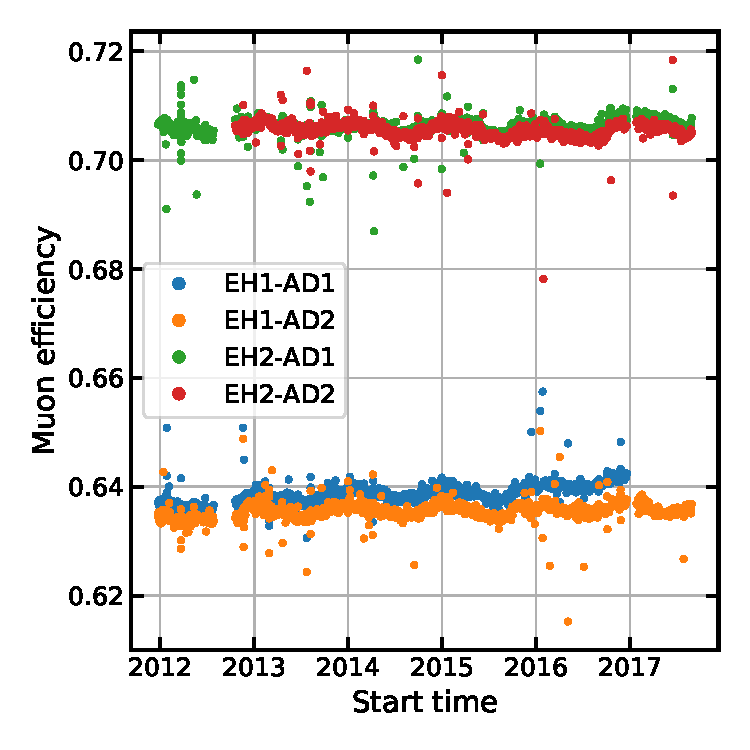
\includegraphics[width=0.48\textwidth]{plot_diagnostics/muon_eff_near_bydate}
    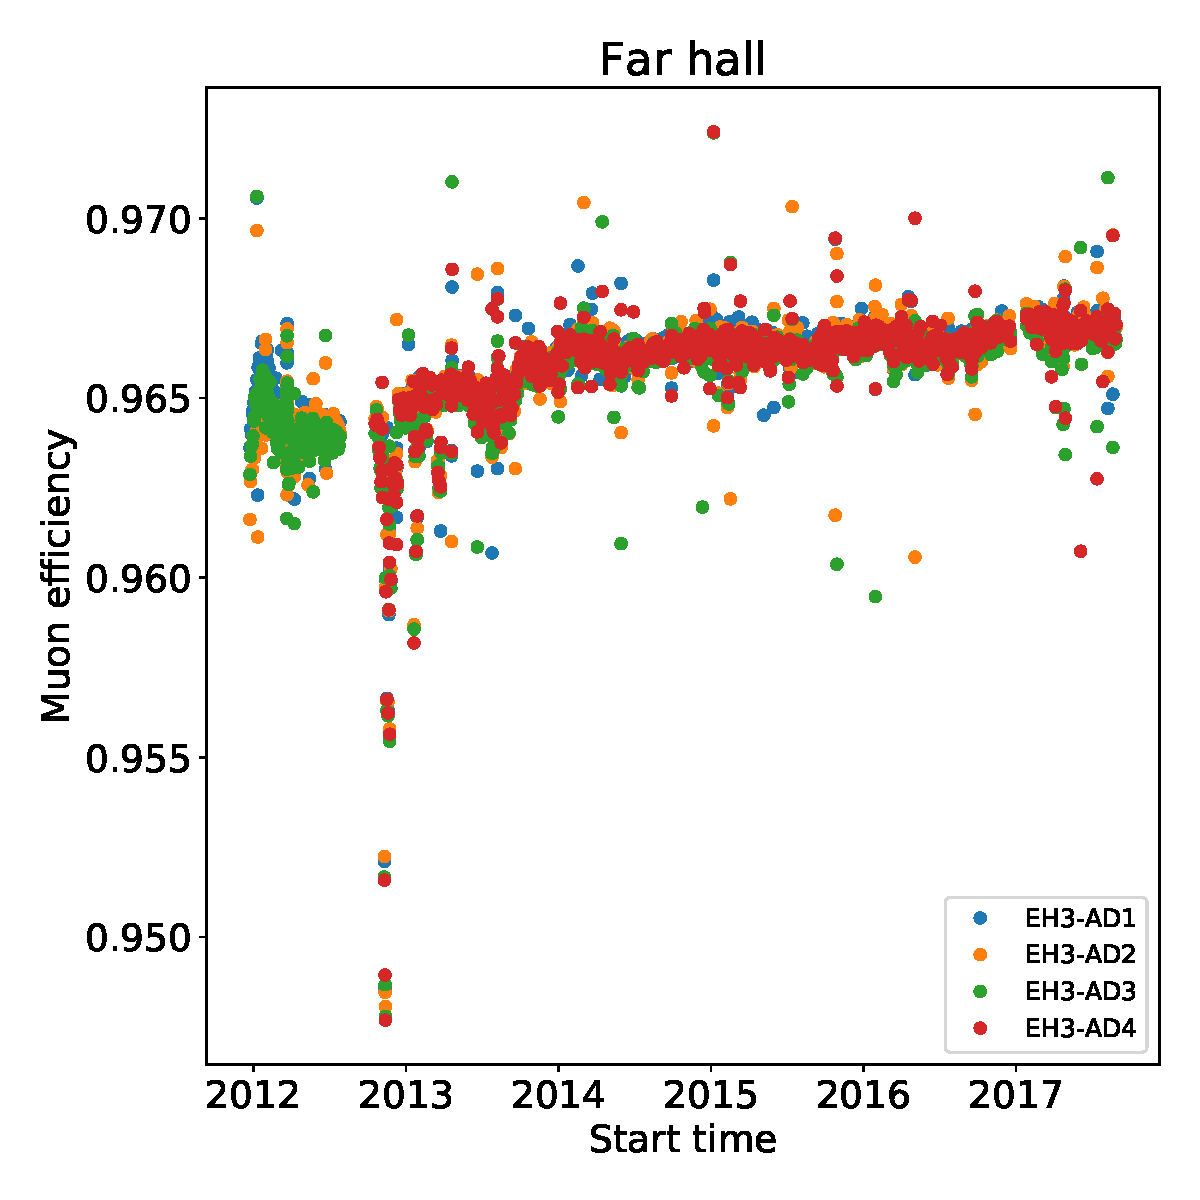
\includegraphics[width=0.48\textwidth]{plot_diagnostics/muon_eff_far_bydate}
    \caption{
        Muon veto efficiency $\varepsilon_\mu$ over time for
        the near halls (left) and far hall (right).
        Each data point represents one data run.
    }
    \label{fig:veto_eff}
\end{figure}

\begin{figure}
    \missingfigure{Effective muon rate}
    \caption{
        Effective muon rate $R_\mu$ over time for the near halls and far hall.
        Each data point represents one data run.
    }
    \label{fig:muon_rate}
\end{figure}

%\section{Initial data preparation}
%\label{sec:dataprep}

%Before physics events are identified,
%major backgrounds that can be cleanly rejected are identified and removed.
%First, events with trigger types not used for the \thetaot{} analysis
%are discarded (see \cref{tab:trigger}).
%This includes random triggers, RPC triggers, and cross triggers.
%Second, cosmogenic muon events are identified
%and a time window after each muon is vetoed
%to allow for any spallation products or activated nuclei to decay
%without contaminating the IBD signal.
%\begin{itemize}
    %\item An IWS event with \num{>12} hit PMTs or an OWS event with \num{>15} hit PMTs
        %is considered a water shield muon.
        %All events in the subsequent \SI{400}{\us} are vetoed.
    %\item An AD event with $E > \SI{20}{\MeV}$ is considered an AD muon.
        %All events in the subsequent \SI{800}{\us} are vetoed.
    %\item An AD event with $E > \SI{2500}{\MeV}$ is considered a showering muon.
        %These muons have created particle showers within the AD,
        %and therefore have a higher probability of creating the activated nuclei
        %\isotope[9]{Li}, \isotope[8]{He}, or \isotope[12]{B}.
        %They occur infrequently enough that
        %all events in the subsequent \SI{1}{\s} can be vetoed
        %without a substantial decrease in livetime efficiency.
%\end{itemize}
%The full details of the muon veto are presented in \cref{sec:muonveto}.

%Next, occurrences of PMT light emission, known as ``flashers,''
%are also vetoed and removed from the data stream.
%These events are caused by sparking in the dynode of the PMT
%and have a geometrical signature in the pattern of hit PMTs.
%The flasher PMT itself observes a high amount of charge,
%as do the PMTs on the opposite wall of the AD,
%due to the directional emission of light from the flasher PMT.
%A cut based on the charge pattern is used to reject flashers
%with a negligible inefficiency for true IBDs.
%The details of the flasher cut are described in \cref{subsec:flashers}.

%Lastly, the vast majority of naturally-occuring radioactivity is rejected
%using an initial energy cut of \SI{1.5}{\MeV}.
%Since the oscillation minumum for Daya Bay occurs at $\sim\SI{3}{\MeV}$,
%this cut preserves the information needed for oscillation measurements.
%Even with low-energy events vetoed, a substantial number of
%uncorrelated radioactive decays are present in the final dataset
%and, when two such decays accidentally occur within a short time window,
%creat the accidental background, which will be discussed in \cref{subsec:acc}.

\section{Flasher events}
\label{sec:flashers}

The high voltage required to operate PMTs rendered them susceptible
to electrostatic breakdown (sparks), also known as flashing.
In the Daya Bay PMTs, flashing was observed
at the PMT base circuit board (\cref{fig:flasher_photo}) \cite{flasherphotos_docdb}.
Although the PMT bases were isolated from the
PMT photocathodes by the black radial shield (\cref{ch:detector}),
light from the spark could propagate within the PMT
or otherwise circumvent the shielding.
These photons created signals at the PMT's own photocathode
or traversed the scintillating region and triggered other PMTs.
Five distinct signatures were observed for flasher events.
\begin{itemize}
    \item ``Nominal flashers.'' Photons activated the flashing PMT's own photocathode,
        creating a large signal.
        Other photons traversed the scintillating region and were incident
        on the PMT's directly across the AD, creating additional large signals.
        Other PMTs observed only small signals.
        Additionally, the shape of the voltage (charge) pulse from the
        flashing PMT was broader than an ordinary signal.
    \item ``2-inch flashers.'' The three 2-inch PMTs in each AD
        used to monitor the scintillators also caused flasher events.
        The signature was a large signal in one of those PMTs.
    \item ``Top-ring flashers.'' Groups of signals were observed
        with reconstructed positions far above the top ring of PMTs
        and outside the scintillating region.
        The physical origin of these flashers is not well understood,
        but one possibility is that light from a flashing PMT
        escapes the base of the PMT
        and passes through a small gap between the radial shield
        and the reflector at the top of the ADs.
        The gap is much smaller at the bottom of the ADs,
        explaining the absence of bottom-ring flashers.
        Another possibility is that these events
        were 2-inch PMTs flashing at a lower energy,
        thus evading the cut used to reject 2-inch flashers.
    \item ``Outside flashers.'' Groups of signals were observed
        with reconstructed positions far outside the scintillating region.
        The physical origin of these flashers is not well understood.
    \item ``Hidden flashers.''
        During investigations of the other types of flasher events,
        groups of signals were observed that survived the existing cuts
        but were suspected to be flashers.
        Their physical origin is poorly understood.
\end{itemize}

Flasher events occasionally generated enough light to be categorized as muon-like.
Events which satisfied both a muon criterion and a flasher criterion
were conservatively treated as muons.

Previous Daya Bay analyses only rejected the first two types of flashers,
nominal and 2-inch flashers,
because the latter three types were accounted for
as part of the uncorrelated background (\cref{sec:acc}).
Additional efforts within the Daya Bay collaboration
to characterize the remaining so-called residual flashers
revealed that these events are not purely uncorrelated,
and so could not be fully accounted for as part of the uncorrelated background.
In particular, the distribution of time delays
between consecutive residual flashers
shows that they are anti-correlated in time:
as shown in \cref{fig:flasher_anticorr},
a residual flasher never flashes twice within $\lesssim \SI{0.7}{\s}$.
The energy distribution of the residual flasher events
limited their relevance to only the nH analysis; the nGd analysis was not affected.
The nominal and 2-inch flasher cuts are described in \cref{subsec:flash_nominal}.
The remaining flasher cuts are described in \cref{subsec:flash_resid}.

\begin{figure}
    \centering
    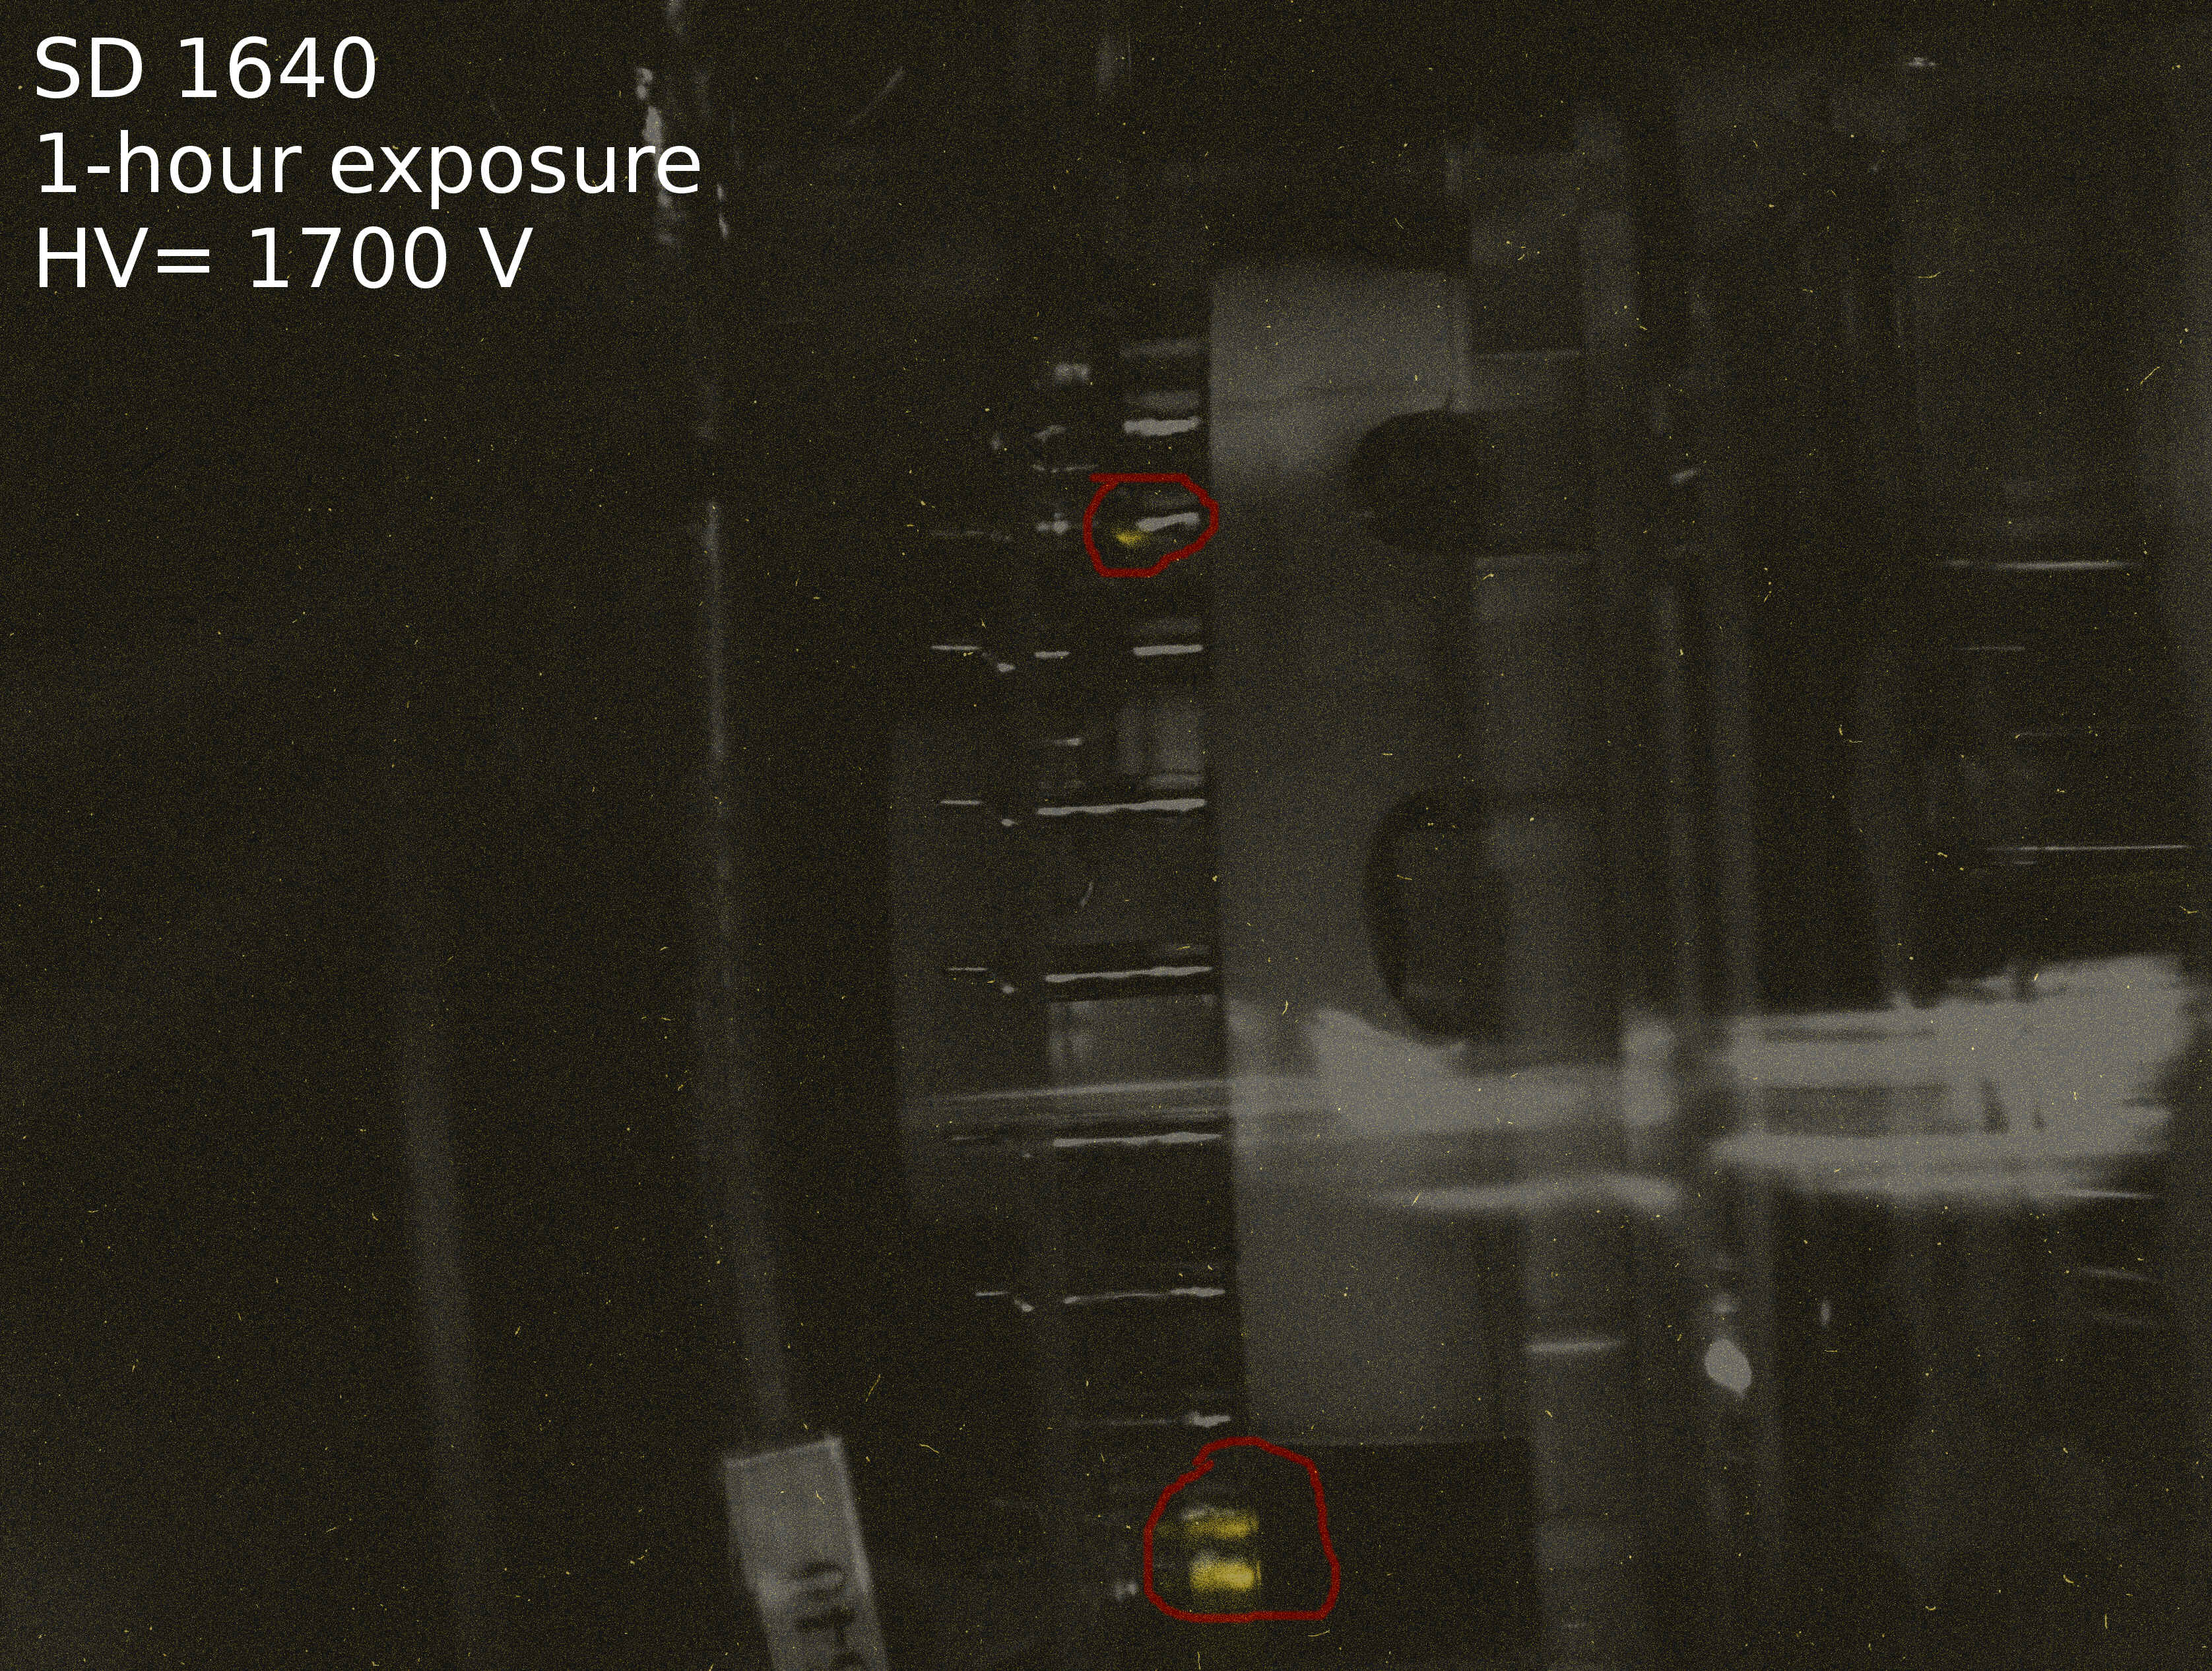
\includegraphics[width=0.8\textwidth]{ch_event_selection/flasher_photo}
    \caption{
        Observation of electrostatic breakdown at the base of a Daya Bay PMT
        \cite{flasherphotos_docdb}
    }
    \label{fig:flasher_photo}
\end{figure}

\begin{figure}
    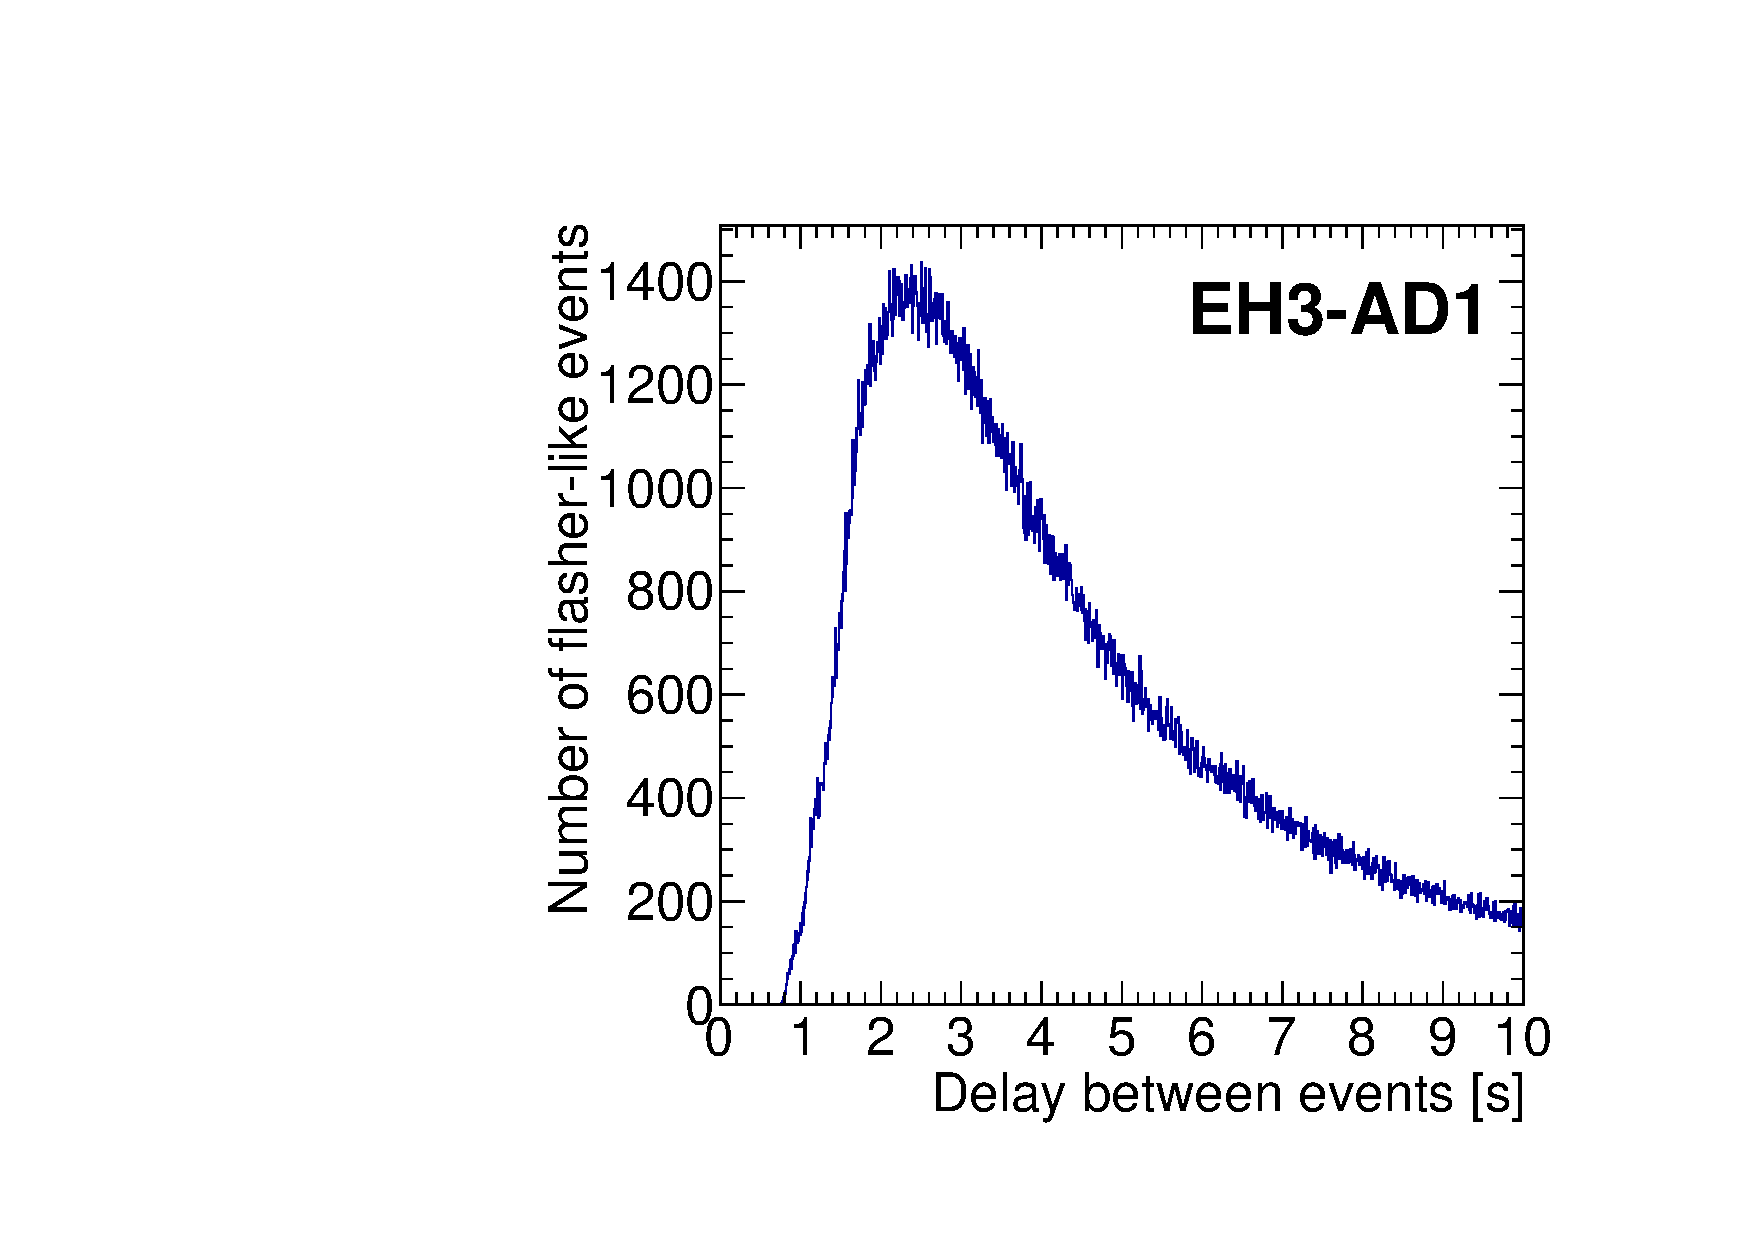
\includegraphics[width=0.48\textwidth]{ch_event_selection/resid_flasher_dt_EH3_AD1}
    \includegraphics[width=0.48\textwidth]{%
        ch_event_selection/resid_flasher_dt_zoomed_EH3_AD1%
    }
    \caption{
        Left: The distribution of time delays
        of a subset of residual flashers in EH3-AD1.
        Right: The same distribution, zoomed in to shorter delays.
        The minimum coincidence time of a residual flasher pair is always
        $\gtrsim \SI{0.7}{\s}$.
        Plots taken from \cite{beda_resid_flasher_dt}.
    }
    \label{fig:flasher_anticorr}
\end{figure}

\subsection{Nominal and 2-inch flasher cuts}
\label{subsec:flash_nominal}

The characteristic event geometry of nominal flasher events
leads to a simple discriminator to reject them on an event-by-event basis.
The flashing PMT itself had by far the largest observed charge
for a flasher event since it was the source of the emitted light.
The emitted photons traveled directly across the AD
and were incident on the PMTs opposite the flashing PMT;
PMTs which were not directly across from the flashing PMT
observed much less light.
The PMT which observed the most charge for each event
was identified as a potential flasher.
A quantity $f_{\text{max}}$ was defined as the fraction of total event charge
which was collected by the potential flasher,
$f_{\text{max}} = Q_{\text{max}}/Q_{\text{total}}$.
For nominal flasher events, $f_{\text{max}}$ was much larger than for ordinary events.
The PMTs were divided into 4 quadrants based on their column in the AD
relative to the potential flasher,
with the potential flasher at the center of Quadrant 1,
and the PMTs opposite the potential flasher assigned to Quadrant 3.
The total charge observed by the PMTs in a given Quadrant $i$
was labeled $Q_i$.
The degree to which the light in an event was focused
opposite the potential flasher
is represented by the quantity $f_{\text{quad}} = Q_3/(Q_2 + Q_4)$,
which is large when more charge is observed in Quadrant 3
relative to the two side quadrants (2 and 4).
The discriminator for nominal flashers was defined as
\begin{equation}
    f_{\text{ID}} = \log_{10}\left(
        f_{\text{Quad}}^2 + \left(
            \frac{f_{\text{max}}}{0.45}
        \right)^2
    \right),
\end{equation}
with $f_{\text{ID}} < 0$ for IBD candidates and other physics events,
and $f_{\text{ID}} > 0$ for nominal flasher events.
As shown in \cref{fig:flasher_nominal_cut},
very few events have $f_{\text{ID}}\sim0$;
it is an effective cut for unambiguously partitioning the set of events.
The few events near the $f_{\text{ID}} = 0$ boundary
are treated in \cref{subsec:flash_resid}.
All nominal flasher-like events (with $f_{\text{ID}} > 0$) were rejected
and were excluded from the coincidence selection.

\begin{figure}
    \missingfigure{MaxQ vs Quadrant plot, and $f_{\text{ID}}$ histogram}
    \caption{
        Left: $f_{\text{max}}$ vs. $f_{\text{quad}}$ for EH1-AD1,
        with the ellipse representing $f_{\text{ID}} = 0$.
        Right: The distribution of $f_{\text{ID}}$ for all ADs.
    }
    \label{fig:flasher_nominal_cut}
\end{figure}

The 2-inch monitor PMTs also caused flasher events.
It was determined that ordinary events (non-flashers)
never deposited more than \SI{100}{\pe} worth of light
in a 2-inch PMT;
events where any 2-inch PMT observed \SI{100}{\pe} or more
were therefore rejected as 2-inch flasher events.
Additional flasher events caused by these PMTs with less than \SI{100}{\pe}
may be the physical origin of top-ring flashers,
discussed in \cref{subsec:flash_resid}.

\subsection{Residual flasher cuts}
\label{subsec:flash_resid}

The remaining three types of flasher events---%
top ring, outside, and hidden flashers---%
were collectively referred to as residual flashers.
Top-ring flashers were easily identified and removed
by rejecting any event with a reconstructed position
of $z > \SI{2.4}{\m}$ and $r^2 > \SI{0.25}{\m\squared}$
(\cref{fig:flash_top_ring}).
(Another variant of this cut uses $r^2 > \SI{0.5}{\m\squared}$.)
The number of true physical single events and
true IBD events removed by this cut was negligible.
Outside flashers were similarly easy to remove
by rejecting any event with a reconstructed position
of $r > \SI{2.2}{\m}$,
again with a negligible inefficiency for singles and IBDs.

The hidden flashers, as the name implies, proved more difficult to isolate.
They were first noticed during an examination of the distribution of distances
between consecutive events.
Sharp peaks were observed in EH3-AD1 at distances of \SIlist{0;2.75;2.9;3.1}{\m},
and in EH3-AD3 and EH3-AD4 at \SI{0}{\m}.
Further inspection of the position distribution of events with these distances
revealed ``hot spots'' within and outside the ADs.
Those events outside the AD were tagged as outside flashers.
To isolate the remaining hidden flashers,
various distributions were explored using the existing flasher-related variables,
including the $f_{\text{ID}}$ parameter and the various quadrant charges $Q_i$.
Eventually, a trapeziod-shaped cut in the parameter space of
$f_{\text{ID}}$ vs. $Q_1/Q_2$ was identified which rejected
$\SI{>80}{\percent}$ of hidden flashers while incorrectly rejecting only
$\sim\SI{0.02}{\percent}$ of true IBDs.
Events which satisfied all of the the following three criteria were rejected:
(1) $Q_1/Q_2 > 0.6$; (2) $f_{\text{ID}} > 0.5 \times Q_1/Q_2 - 0.8$;
and (3) $f_{\text{ID}} > 0.3$,
as illustrated in \cref{fig:hidden_flasher_cut}
\cite{flashers_jinjing,beda_resid_flasher_dt}.
The estimated rate of residual flashers over time for each AD is shown
in \cref{fig:hidden_flasher_rate}.


\begin{figure}
    \missingfigure{Top-ring flashers position}
    \caption{
        Position distribution of single events in EHX-ADY,
        with the top-ring flashers clearly visible at $z > \SI{2.4}{\m}$.
    }
    \label{fig:flash_top_ring}
\end{figure}

\begin{figure}
    \missingfigure{$Q_1/Q_2$ vs ellipse ``hidden'' flasher cut plot}
    \caption{
        Distribution of events in $Q_1/Q_2$-$f_{\text{ID}}$ space.
        The events within the black outline are vetoed as
        hidden flashers.
        Events above $f_{\text{ID}}=0$ are already vetoed as nominal flashers.
    }
    \label{fig:hidden_flasher_cut}
\end{figure}

\begin{figure}
    \missingfigure{Hidden flasher rate over time}
    \caption{
        Rate of hidden flashers over time for each AD.
    }
    \label{fig:hidden_flasher_rate}
\end{figure}


\section{Coincidence selection}
\label{sec:coincidence}

Events are grouped based on the number of other events
occuring within a given coincidence time \tc.
Each event with reconstructed energy above \SI{1.5}{\mega\electronvolt}
is identified as an ``AD event''
and is a potential coincidence candidate.
Because of the nonzero length of the DAQ readout window,
AD events occurring closer together than \SI{1}{\micro\second}
are not necessarily distinct physical events (see \cref{sec:daq}).
\todo{How frequently are 2 ``events'' so close?}
Consequently, during the coincidence grouping process,
the coincidence search window begins \SI{1}{\micro\second}
after the initial AD event.
Coincidence groups are constructed by repeating the following steps
(illustrated in \cref{fig:timeline_examples}) until the data file is exhausted \cite{thucoinc2015}:

\begin{enumerate}
    \item Find the next AD event.
        This AD event will be the ``prompt'' event of the coincidence group.
    \item Find all subsequent AD events within the desired coincidence time \tc.
        If a muon event is encountered within \tc,
        veto the entire coincidence group starting with the prompt event.
        (This additional vetoed time is accounted for in the muon veto efficiency.)
    \item Group these events together with the prompt event
        to form the coincidence group.
    \item Skip to the next AD event that is not part of the coincidence group.
\end{enumerate}

\begin{figure}
    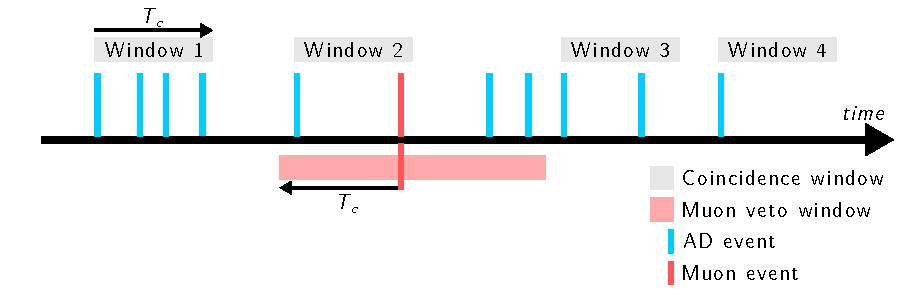
\includegraphics{ch_event_selection/timeline_examples}
    \caption{
        An example timeline showing how coincidence groups are created,
        and how they interact with muons and muon veto windows.
        This illustration does not show the \SI{1}{\micro\second} gap
        at the start of each coincidence window.
        Windows 1, 3, and 4 are valid coincidence groups,
        while Window 2 is vetoed by the muon event.
    }
    \label{fig:timeline_examples}
\end{figure}

Because of the initial \SI{1}{\micro\second} gap,
the actual time interval covered by any given coincidence window is
$\tc - \SI{1}{\micro\second}$.
This analysis uses a coincidence search window of $\tc = \SI{1.5}{\milli\second}$.

The total number of AD events in the group
is the multiplicity of the group.
A coincidence group with multiplicity $n$ is also referred to
as an \fold{n} coincidence.
In Window 1 of \cref{fig:timeline_examples},
the first AD event starts a new coincidence window
that includes three other AD events,
resulting in a coincidence group of multiplicity 4, or a \fold{4} coincidence.

If a muon event occurs within a coincidence window,
then that coincidence window is vetoed.
Therefore every muon has an implicit veto window
that excludes prompt events within \tc{} of the muon.
This is demonstrated by Window 2 of \cref{fig:timeline_examples}.
Note that if the prompt event occurs earlier than \tc{} before a muon,
then subsequent events within the coincidence window
are allowed to occur inside of the implicit muon veto window.
Only prompt events are vetoed by the implicit veto window.

The veto window after a muon also impacts the coincidence selection process.
Window 3 of \cref{fig:timeline_examples} shows a coincidence window
whose prompt event is preceded by other recent AD events.
However, those AD events fall within the previous muon veto window,
so they are ignored for the purposes of forming coincidence groups.

If a prompt event has no subsequent AD events within \tc, it is
still a valid group, and is referred to as a \fold{1} coincidence.
Note that \fold{1} coincidences are somewhat but not strictly isolated
from other AD events.
Certainly there are no other AD events
within \tc{} \textit{after} the prompt event,
but there may be a \textit{preceding} AD event within \tc{}
if that event is part of a coincidence window
which ends before the prompt event in question.
Window 4 of \cref{fig:timeline_examples} demonstrates this property:
there are no other AD events within Window 4,
but there is a previous AD event within \tc{} of the start of Window 4.
Given the event rates at Daya Bay, this only happens in $\sim10^{-4}$
of single events.
This probability is derived in \cref{ap:singlesformula} as $P_b$.


\adgrid{All double coincidences found using $\tc=\SI{1.5}{\milli\second}$}{fig:double_coinc_raw}{ch_event_selection/double_coincs}

Once the coincidence groups have been constructed,
the set of \fold{2} coincidences
contains IBD candidates
with substantial background still present.
With a coincidence time of $\tc=\SI{1.5}{\ms}$
and a neutron capture time of $\sim\SI{200}{\us}$ in LS,
there is a negligible inefficiency due to neutrons
which take longer than \tc{} to capture on hydrogen.
\Cref{fig:double_coinc_raw} shows the prompt and delayed energy
of all \fold{2} coincidences identified each AD.
These plots clearly show the nGd events
at delayed energy values near \SI{8}{\mev}.
The nH events are visible as the narrow band at
delayed energies near \SI{2.2}{\mev}
and prompt energies of \SIrange{4}{7}{\mev}.
At prompt energies less than \SI{3.5}{\mev} or greater than \SI{7}{\mev}
these signal events are overwhelmed by the accidental background,
which is characterized in these plots by the 4-point square at both prompt and
delayed energies of \SIlist{1.5;3.25}{\mev}.

\begin{figure}
    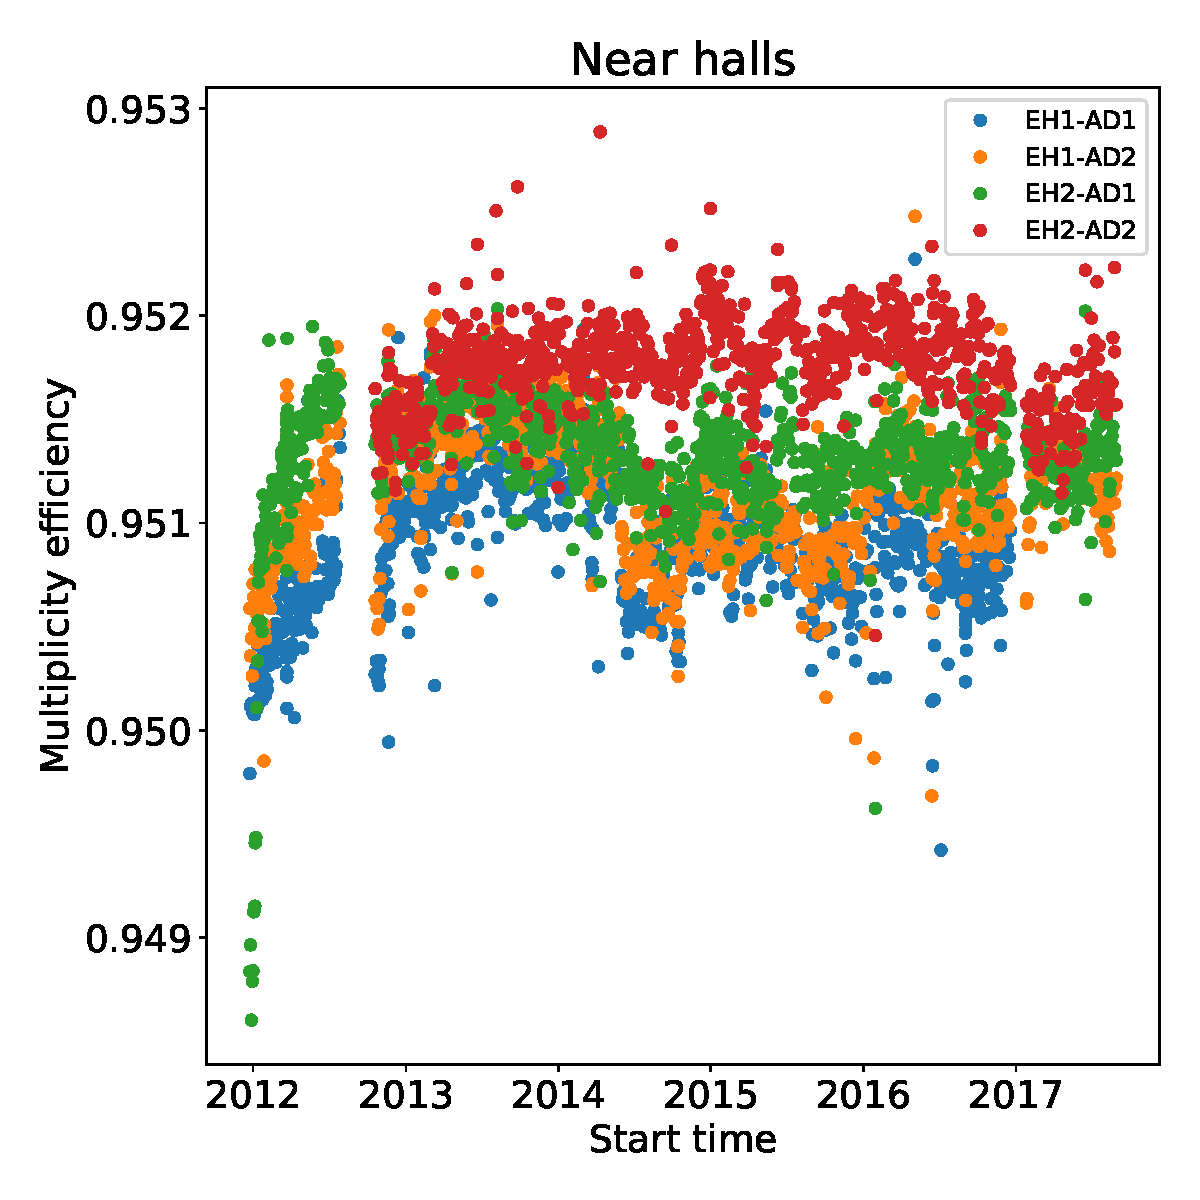
\includegraphics[width=0.48\textwidth]{plot_diagnostics/mult_eff_near_bydate}
    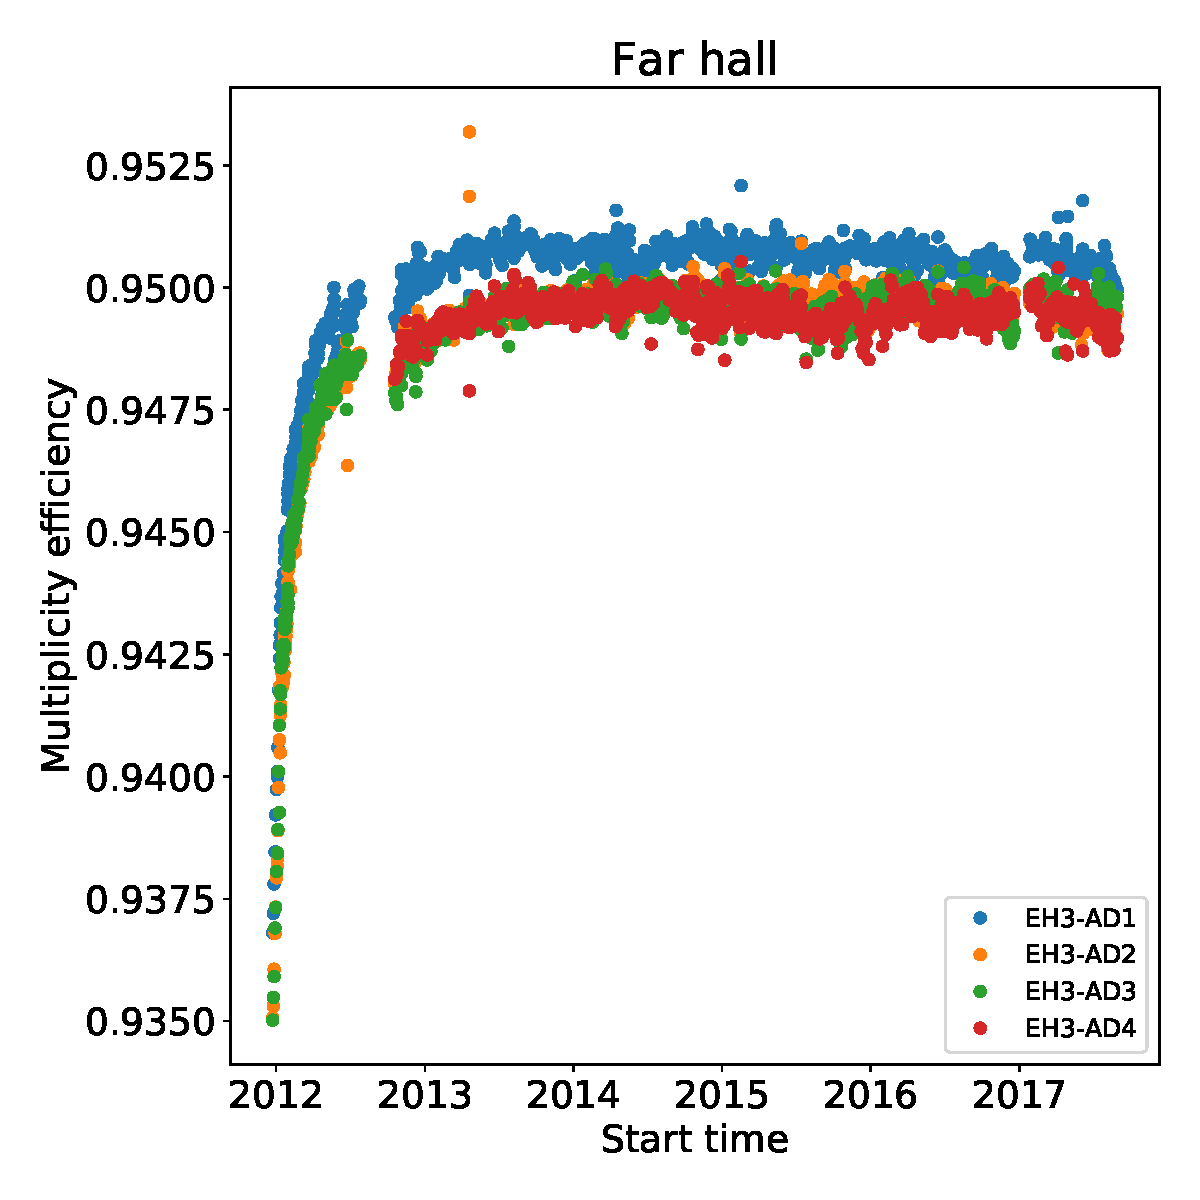
\includegraphics[width=0.48\textwidth]{plot_diagnostics/mult_eff_far_bydate}
    \caption{
        Multiplicity veto efficiency $\varepsilon_m$ over time for
        the near halls (top) and far hall (bottom).
        Each data point represents one data run.
    }
    \label{fig:mult_eff}
\end{figure}
The set of \fold{1} coincidences is a subset
of the uncorrelated events, mostly radioactive decays,
that are also present in the data stream.
However, not all uncorrelated events end up in \fold{1} coincidences.
Sometimes an uncorrelated event will occur in close time proximity to
a true IBD prompt-delayed pair, creating a \fold{3} coincidence.
These high-multiplicity coincidence groups are vetoed
with a small loss of efficiency.
The efficiency of this multiplicity cut is derived in \cref{ap:singlesformula} as
\cref{eq:mult_eff_ap}:

\begin{align}
    \label{eq:mult_eff}
    \begin{split}
        \varepsilon_m &= e^{-R_s \tc}
        \left(
            e^{-(R_s + R_\mu)\tc} +
            \frac{R_s}{R_s+R_\mu} e^{-R_\mu\tc}
            \left(
                1 - e^{-(R_s + R_\mu)\tc}
            \right)
        \right. \\
              &\ \ \left. - \frac{R_s}{2R_s + R_\mu} e^{-R_\mu\tc}
                  \left(
                      1 - e^{-(2R_s + R_\mu)\tc}
                  \right) +
                  \frac{R_\mu}{R_s + R_\mu}
                  \left(
                      1 - e^{-(R_s + R_\mu)\tc}
                  \right)
              \right),
    \end{split}
\end{align}
where $R_s$ is the rate of uncorrelated events,
$R_\mu$ is the effective muon rate,
and \tc{} is the length of the coincidence window, \SI{1499}{\us}.
The multiplicity efficiency over time is shown in \cref{fig:mult_eff}.
More concerning is when two uncorrelated events
randomly occur in close proximity to each other,
creating a \fold{2} coincidence group that passes the multiplicity veto.
These so-called ``accidental'' coincidences
constitute the largest background within the set of \fold{2} coincidences
(\cref{sec:acc}).
The distance, time and energy cuts described below
are all motivated in large part by the need to reduce the accidental background.

\section{Distance and time cuts}
\label{sec:DT_cut}

The characteristic distance for a neutron capture on hydrogen
is approximately \SI{200}{\milli\meter},
and the characteristic time delay is \SI{\sim215}{\us}.
For accidental coincidences, the characteristic distance is
the length scale of the AD, approximately \SI{3000}{\milli\meter},
and the characteristic time based on the \fold{1} event rate
is $\sim\SI{50000}{\us}$.
%On the time scale of the coincidence window length $\tc=\SI{1500}{\us}$,
%any particular coincidence time is approximately equally probable.

\adgrid{Distribution of coincidence distance and coincidence
time\todo[inline]{Fix y axis tick labels}}{fig:dr_vs_dt}{ch_event_selection/dr_vs_dt}

\Cref{fig:dr_vs_dt} shows the distribution of
coincidence distance and coincidence time
for the subset of \fold{2} coincidences with
relatively small coincidence distances and times
of less than \SI{1000}{\milli\meter} and \SI{600}{\micro\second},
respectively.
The cluster at the lowest coincidence times and distances
consists of IBD events.
The rest of the events distributed with relatively uniform density
across the plot are accidental coincidences from uncorrelated events.
This plot was used as a heuristic to determine a distance and time cut
by drawing a line from \SI{800}{\milli\meter} at $0$ time
to \SI{480}{\micro\second} at $0$ distance.
This line effectively separates the higher-density region
of correlated events from the uniform density region of accidental background.
The distance-time (DT) cut is defined by this line,
and accepts events which satisfy the inequality
\begin{equation}
    \text{DT} = \Delta r + v_0 \Delta t < \SI{800}{\milli\meter},
\end{equation}
where $v_0 = \frac{\SI{1000}{\milli\meter}}{\SI{600}{\micro\second}}$.
Note that the quantity DT is not D$\times$T,
nor should it be confused the differential $dt$.
\Cref{fig:after_DT_cut} shows the individual AD spectra
after applying the DT cut.
As expected, the accidental background present
in the low-prompt-energy and low-delayed-energy corner has been reduced.
The neutron capture on hydrogen events now stand out much better
against the accidental background.

\adgrid{Prompt-delayed energy spectra after applying
the DT cut}{fig:after_DT_cut}{ch_event_selection/post_DT_cut}

Applying the DT cut rejected the vast majority of accidental events
at a loss of approximately \SI{30}{\percent} of real IBDs.
The absolute efficiency was defined as
\begin{equation}\label{eq:abs_DT_eff}
    \varepsilon_{\text{DT}} = \frac{
        N_\text{IBD}[E_p \wedge E_d \wedge \text{DT}]
    }%
    {
        N_\text{IBD}[E_p \wedge E_d]
    },
\end{equation}
the fraction of IBD events passing the prompt and delayed energy cuts
which also pass the DT cut.
This value was estimated by constructing a 2D histogram
showing the DT parameter and delayed energy value
for all double coincidence events.
A separate histogram was constructed using the same quantities
but for the synthetic accidental background events, described in \cref{sec:acc}.
The accidentals histogram was normalized so that
\begin{equation}\label{eq:acc_sub_normalized}
    \int_{E_d}\int_{\SI{3}{\m}}^{\SI{10}{\m}}
    \frac{d^2N_\text{obs}}{dE_d d(\text{DT})}
    dE_d d(\text{DT})
    =
    \int_{E_d}\int_{\SI{3}{\m}}^{\SI{10}{\m}}
    \frac{d^2N_\text{acc}}{dE_d d(\text{DT})}
    dE_d d(\text{DT})
\end{equation}
based on the assumption that all observed events
with a DT parameter greater than \SI{3}{\m}
were accidental coincidences.
Subtracting the accidentals histogram from the observed double coincidences
thus provided the distribution of correlated events
(true IBDs as well as correlated backgrounds)
as a function of delayed energy and DT parameter,
denoted $N_\text{sub}$.
By construction,
\begin{equation}\label{eq:acc_sub_normalized_zero}
    \int_{E_d}\int_{\SI{3}{\m}}^{\SI{10}{\m}}
    \frac{d^2N_\text{sub}}{dE_d d(\text{DT})}
    dE_d d(\text{DT})
    = 0.
\end{equation}
A further assumption, that the position distribution of correlated backgrounds
(most of which involved a prompt event followed by nH capture)
was equal to the position distribution of IBDs,
was made to allow the approximation of \cref{eq:abs_DT_eff} as
\begin{equation}\label{eq:abs_DT_eff_approx}
    \varepsilon_{\text{DT}} \approx \frac{
        N_\text{sub}[E_p \wedge E_d \wedge \text{DT}]
    }%
    {
        N_\text{sub}[E_p \wedge E_d]
    }.
\end{equation}
\Cref{fig:ed_DT_sub} illustrates how the DT cut efficiency is measured
for each AD using a histogram of delayed energy and DT value
to determine the number of events which pass the nominal and relaxed DT cuts.
The measured DT cut absolute efficiency for each AD is shown in \cref{fig:DT_eff}.
Like all absolute detection efficiencies,
$\varepsilon_{\text{DT}}$ was not used as an input to the \thetaot{} analysis.
However, the variation between ADs was treated as the AD-uncorrelated uncertainty
of the detection efficiency due to the DT cut.
The \SI{>3}{\percent} apparent variation between ADs
motivated additional investigation
to determine whether the variability was intrinsic to the ADs
or was simply an artifact of one or more of the assumptions
used to extract the efficiency values.

The extraction of the absolute efficiency was extremely sensitive
to small variations in the accidentals subtraction procedure.
The sensitivity arose when computing $N_\text{sub}[E_p \wedge E_d]$
Most of the range of DT values was characterized by
very few correlated events but many accidental coincidences.
A change of \SI{0.01}{\percent} in the normalization (rate)
of the subtracted background at a far site AD
yielded a relative impact of \SI{2.1}{\percent} in the extracted DT cut efficiency,
amplifying the bias by a factor of over 200.
(The near site ADs were sensitive by a factor of $\sim30$.)
Normalizing the high-DT range of the distributions,
as shown in \cref{eq:acc_sub_normalized},
addressed most of this issue,
but the precise choice of lower bound
could still impact the computation
due to statistical fluctuations in the histogram bins near $\text{DT} = \SI{3}{\m}$.

Two special selections were used to reduce the impact of
the accidentals subtraction procedure on the DT cut efficiency uncertainty.
The first selection consisted of events where the neutron captured on Gd
rather than H.
They were isolated using the plots shown in \cref{fig:ed_DT_sub}
by selecting the region with delayed energy between \SIlist{6;12}{\MeV}.
The second selection consisted of nH events
with a prompt energy above \SI{3.5}{\MeV}.
The accidentals-subtracted plots of delayed energy versus DT were
modified to only include events with $E_p > \SI{3.5}{\MeV}$,
and the DT efficiency procedure was repeated.
The same delayed energy cut was used for this modified sample
as for the nominal sample.
The nGd subset yielded a full range of \SI{0.18}{\percent}
in DT cut absolute efficiencies between ADs,
while the $E_p > \SI{3.5}{\MeV}$ yielded a full range of \SI{0.94}{\percent}.
The extracted efficiencies for each AD are shown in \cref{fig:DT_eff_subsamples}.
Between these two subsets, almost the entire range
of prompt and delayed positions and energies used in the nominal selection was represented,
allowing the DT cut efficiency uncertainty to be accurately estimated
with a minimal impact from the accidental background.
Conservatively, the half-range of the $E_p > \SI{3.5}{\MeV}$ subset,
\SI{\pm0.47}{\percent}, was
used as the AD-uncorrelated uncertainty of the DT cut efficiency.

\begin{figure}
    \missingfigure{DT efficiency subsamples: nGd and $E_p > \SI{3.5}{\MeV}$}
    \caption{
        Extracted DT cut efficiencies for the subsample of events
        with neutron capture on nGd and with prompt energy
        greater than \SI{3.5}{\MeV}.
    }
    \label{fig:DT_eff_subsamples}
\end{figure}

\begin{figure}
    \centering
    \includegraphics[width=0.49\textwidth, trim={0 0 0 1cm}, clip]{%
        ch_event_selection/ed_DT_sub_EH1_AD1%
    }
    \includegraphics[width=0.49\textwidth, trim={0 0 0 1cm}, clip]{%
        ch_event_selection/ed_DT_sub_EH2_AD1%
    } \\
    \includegraphics[width=0.49\textwidth, trim={0 0 0 1cm}, clip]{%
        ch_event_selection/ed_DT_sub_EH3_AD1%
    }
    \caption{
        Accidentals-subtracted distribution of
        delayed energy and DT value, used to compute $\varepsilon_{\text{DT}}$.
        The green (solid) box shows the events included in the DT cut.
        The black (dashed) box shows the events excluded by the DT cut.
        The large fluctuations at high DT are due to the statistics
        of subtracting two almost-equal large numbers as part of the
        background subtraction procedure.
        \todo[inline]{Update DT efficiency 2D histogram plots}
    }
    \label{fig:ed_DT_sub}
\end{figure}

\begin{figure}
    \centering
    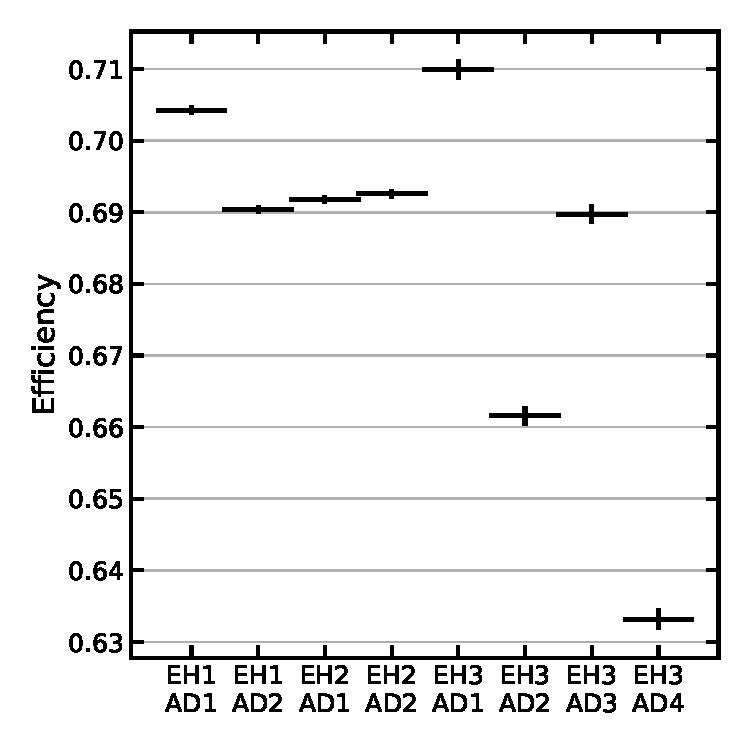
\includegraphics[height=0.4\textheight]{plot_diagnostics/distance_time_cut_efficiency}
    \caption{
        The DT cut efficiency for each AD. Error bars are statistical.
        \todo[inline]{Explain {\em very} clearly or remove}
    }
    \label{fig:DT_eff}
\end{figure}

\section{Accidental coincidences}
\label{sec:acc}

Once muon events and flashers have been removed from the data stream,
the vast majority of remaining AD events are caused by uncorrelated
natural radioactive decays and are commonly known as ``singles,''
although as will be shown shortly, this name is misleading,
and a more appropriate name is ``uncorrelated events.''
These events occur at approximately \SI{19}{\hertz} in each AD
(for energies above \SI{1.5}{\MeV})
and,
because they are uncorrelated, their groupings in time follow Poisson statistics.
In particular, there is a nonzero probability that
two of these uncorrelated ``single'' events will occur within
$\tc=\SI{1.5}{\milli\second}$ and thus form a \fold{2} coincidence.
For any given uncorrelated event, the probability that
another uncorrelated event will occur within \tc{} is

\begin{equation}
    \text{Poisson}(1\vert R_s\tc) = R_s\tc e^{-R_s\tc}.
\end{equation}
For the above value for $R_s=\SI{19}{\hertz}$, this probability is \SI{2.77}{\percent}.
Since \fold{2} coincidence groups like this are not formed from any
deliberate physical proccess but rather by an accidental coincidence,
they are known as the accidental background.
Crucially, though almost all \fold{1} coincidence groups
consist of a single uncorrelated event,
not all uncorrelated events form \fold{1} coincidences.
These so-called ``singles'' are not always lone events.
A back-of-the-envelope estimate of the rate of accidental coincidences gives
$\SI{19}{\hertz}\times\SI{2.77}{\percent}=\SI{0.53}{\hertz}$
before applying the distance-time (DT) cut (\cref{sec:DT_cut}).

\subsection{Uncorrelated events}
\label{subsec:singles}

The full accidentals subtraction procedure begins with identifying
the rate of uncorrelated events in the AD, again better known
as the ``singles rate,'' for each individual data run.
The singles rate is computed by first measuring the rate of
\fold{1} coincidences in each run
(with the prompt energy bound of \SIrange{1.5}{12}{\mev} from \cref{subsec:prompt_energy}).
Given that rate, the true underlying rate of uncorrelated events can be
computed by numerically solving the following formula
(derived in \cref{ap:singlesformula}) for $R_s$:

\begin{align}
    \label{eq:rsingles}
    \begin{split}
        R_{\text{\fold{1}}}
          &= R_s e^{-R_s\tc}
          \left(
              e^{-(R_s + R_\mu)\tc} +
              \frac{R_s}{R_s+R_\mu} e^{-R_\mu\tc}
              \left(
                  1 - e^{-(R_s + R_\mu)\tc}
              \right)
          \right. \\
          &\ \ %
          \left. - \frac{R_s}{2R_s + R_\mu} e^{-R_\mu\tc}
              \left(
                  1 - e^{-(2R_s + R_\mu)\tc}
              \right) +
              \frac{R_\mu}{R_s + R_\mu}
              \left(
                  1 - e^{-(R_s + R_\mu)\tc}
              \right)
          \right)
    \end{split}
\end{align}
In this formula, \tc{} represents the actual duration of the coincidence window,
which technically begins \SI{1}{\micro\second} after the event,
meaning that a value of $\tc=\SI{1499}{\micro\second}$ should be used (\cref{sec:daq}).
This formula is valid under the assumption that all
events in the data stream are truly uncorrelated in time.
Residual flashers are anti-correlated in time
but are vetoed from the data stream (\cref{sec:flashers}).
Correlated events (both IBDs and other backgrounds)
have a rate much smaller than the uncorrelated event rate
($\nicefrac{R_{corr}}{R_s} \sim \num{5e-3}$)
and have a negligible impact on the probability of a \fold{1} coincidence.
\todo{Verify impact on R\_s}

The terms in brackets together represent the probability
that any given event does not fall in another event's coincidence window.
The leading term is simply the uncorrelated event rate $R_s$ times
the Poisson probability that no other uncorrelated event will occur
inside the given coincidence window.

\begin{figure}
    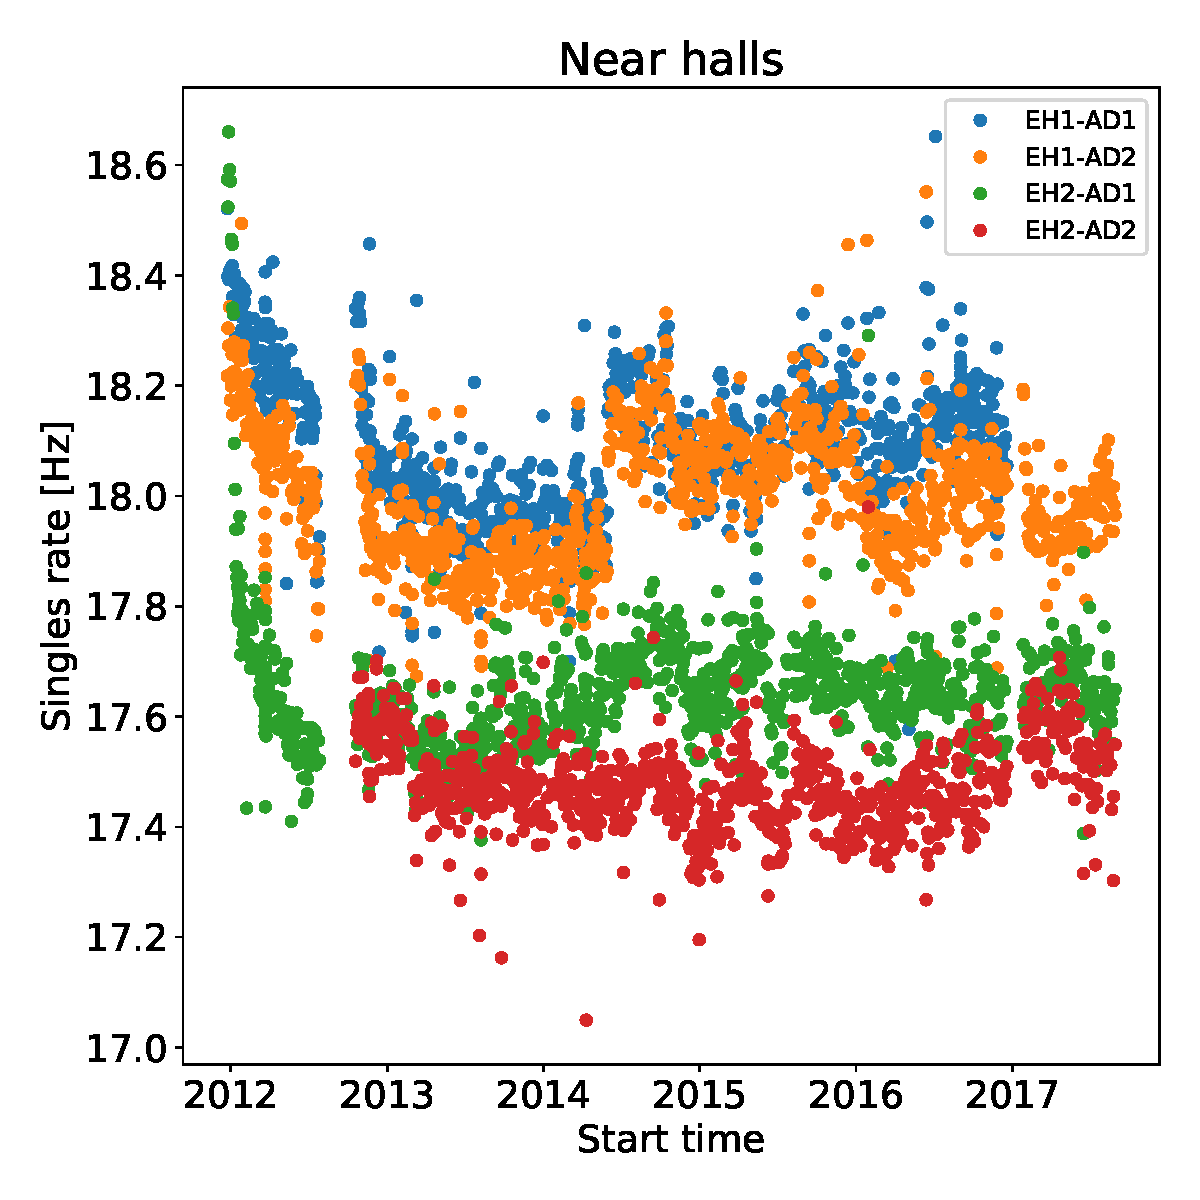
\includegraphics[width=0.48\textwidth]{plot_diagnostics/singles_near_bydate}
    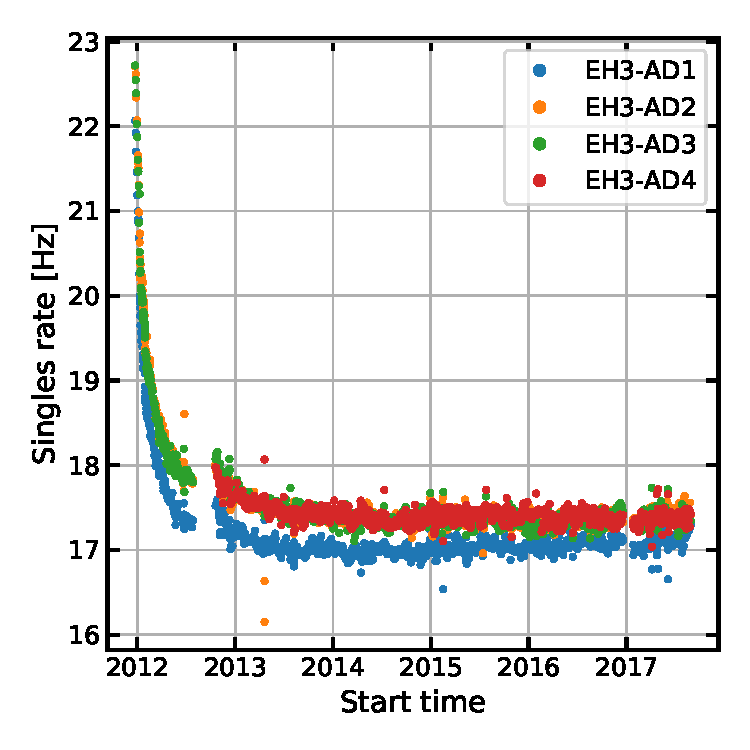
\includegraphics[width=0.48\textwidth]{plot_diagnostics/singles_far_bydate}
    \caption{
        Singles rate $R_s$ over time for
        the near halls (top) and far hall (bottom).
        Each data point represents one data run.
    }
    \label{fig:singles}
\end{figure}

The uncorrelated event rate $R_s$ for the near and far halls is shown in
\cref{fig:singles}.
$R_s$ was higher when the experiment began because long-lived
radioactive contaminants had not yet decayed away.
In particular, the far-hall ADs EH3-AD1, EH3-AD2, and EH3-AD3
were filled shortly before physics data taking began,
while the near-hall ADs EH1-AD1, EH1-AD2, and EH2-AD1
were filled and then studied for a few months
as part of detector commissioning, during which time
most of the radiocontaminants decayed.

Once $R_s$ is obtained, the rate of accidental coincidences $R_{\text{\fold{2}}}$
(before applying the rest of the event selection)
can be computed for each run
by simply adjusting the Poisson probability in \cref{eq:rsingles}
from the probability of $0$ other events within \tc{}
to the probability of $1$:

\begin{align}
    \label{eq:racc}
    \begin{split}
        R_{\text{\fold{2}}} &= R_s\tc R_{\text{\fold{1}}} \\
                   &= R_s \left(R_s\tc e^{-R_s\tc}\right)
          \left(
              e^{-(R_s + R_\mu)\tc} +
              \frac{R_s}{R_s+R_\mu} e^{-R_\mu\tc}
              \left(
                  1 - e^{-(R_s + R_\mu)\tc}
              \right)
          \right. \\
          &\ \ %
          \left. - \frac{R_s}{2R_s + R_\mu} e^{-R_\mu\tc}
              \left(
                  1 - e^{-(2R_s + R_\mu)\tc}
              \right) +
              \frac{R_\mu}{R_s + R_\mu}
              \left(
                  1 - e^{-(R_s + R_\mu)\tc}
              \right)
          \right)
    \end{split}
\end{align}
The rate $R_{\text{\fold{2}}}$ obtained from this formula
cannot simply be subtracted from the measured \fold{2} rate
to obtain $R_{\text{IBD}}$.
Corrections still need to be made to account for
the coincidence distance and time properties of accidentals
as well as the energy spectrum
before the rates can be subtracted.

Like the rate computation, the energy spectrum of accidentals is determined for each run
by focusing on isolated events.
However, unlike the rate, a stricter isolation cut is used
to better ensure that only truly uncorrelated events are included in the sample.
This is acceptable because the characteristics of uncorrelated events
by definition do not change based on the presence or absence
of surrounding events.
A symmetrical isolation cut of $\tc=\SI{1.5}{\milli\second}$ is used
to ensure isolation before and after each candidate event.
The spectrum of these (now truly) single events is shown in \cref{fig:singlespectra},
obtained by summing the individual spectra from each data run.

\adgrid{Spectra of isolated single events in each AD.}{fig:singlespectra}{%
    ch_background/singles%
}

Uncorrelated events are not uniformly distributed
in position within the ADs.
Many of the radiocontaminants are on the surfaces of the
acrylic vessels that separate the mineral oil, LS, and GdLS regions.
To most accurately model the accidental background,
the singles sample is used to create a synthetic sample of accidental coincidences,
which is then used to actually perform the background subtraction
on the IBD candidates data set.
The synthetic accidental coincidence samples are formed for each run
by pairing up isolated events.
In particular, each isolated event is assigned an index in time order,
from $0$ to $N_{\text{isolated}}$.
Then each event $i$ from the first half is paired up with
the corresponding event from the second half, $i + \nicefrac{N_{\text{isolated}}}{2}$.
The coincidence distance is taken to be the actual distance
between the reconstructed positions of the two events.
Each event pair generates two synthetic accidental events:
one with the event from the first half of the run as the prompt event,
and one with that event as the delayed event.
For each ordering and for each event pair, a coincidence time is chosen
uniformly at random to match the coincidence time distribution
expected from true accidental coincidences on the short timescale
of $\tc=\SI{1.5}{\milli\second}$.
From this synthetic accidental coincidence sample, $\varepsilon_{\text{DT,\,acc}}$,
the fraction of accidental \fold{2} coincidences which pass the distance-time (DT) cut,
can be computed.
At this point in the event selection procedure,
the prompt energy cut is known and fixed at \SIrange{1.5}{12}{\MeV}
but the delayed energy cut is still undetermined (\cref{sec:energy_cuts}).
After the delayed energy cut is extracted, $\varepsilon_{\text{total,\,acc}}$,
the fraction of accidental \fold{2} coincidences
which pass the full IBD selection including energy cuts,
is computed.
A prompt-delayed energy spectrum was computed that only includes
synthetic accidental events which passed the DT cut,
as shown in \cref{fig:acc_sample}.
\adgrid[0.22\textheight]{
    Prompt-delayed spectra of the synthetic accidentals sample
    after applying the DT cut.
    Each 2D plot is symmetrical under interchange of prompt and delayed energy
    by construction, since each synthetic pair is added to the histogram twice.
    The plots may not appear to be perfectly symmetrical
    due to artifacts of the plotting software.
}{fig:acc_sample}{ch_background/acc}

The resulting prompt-delayed energy spectrum of synthetic accidental events
can then be subtracted
from the prompt-delayed spectrum measured from real data.
For each run, the expected number of accidental coincidences
with prompt and delayed energies between \SIlist{1.5;12}{\MeV}
that pass the DT cut is

\begin{equation}
    N_{\text{acc,\,loose}} = R_{\text{\fold{2}}} \times t_{\text{muon-corrected}}
        \times \varepsilon_{\text{DT,\,acc}}
    \label{eq:nacc_loose}
\end{equation}
The synthetic accidentals prompt-delayed spectrum, represented as a histogram,
is scaled so that the integral is $N_{\text{acc,\,loose}}$.
Then the histogram can be subtracted bin-by-bin from the corresponding histogram
representing the actual \fold{2} coincidence data sample.
The subtracted histograms are shown in \cref{fig:acc_sub_spectra}.
These distributions, projected onto the delayed energy axis,
are used in \cref{subsec:delayed} to determine the delayed energy cut bounds.

\adgrid[0.22\textheight]{
    Prompt-delayed spectra after subtracting the accidental background.
    The projections of these plots onto the delayed energy axis
    are used to determine the delayed energy cut bounds
    and are shown in \cref{fig:delayed_fits}.
}{fig:acc_sub_spectra}{ch_background/sub_energy}

The scale factor for the accidentals spectrum histogram,
$\frac{N_{\text{acc,\,loose}}}{N_{\text{isolated}}/2}$,
can be used to create histograms for other accidentals-subtracted quantities,
such as coincidence distance and DT, as well as 2D histograms of
those quantities' distributions with respect to prompt and delayed energy.
The accidentals-subtracted histogram of DT versus delayed energy
was used to compute the efficiency of the DT cut for IBDs in \cref{sec:DT_cut}.

The total expected number of accidental events
that pass the full IBD selection is computed in a similar manner:

\begin{equation}
    N_{\text{acc}} = R_{\text{\fold{2}}} \times t_{\text{muon-corrected}}
        \times \varepsilon_{\text{total,\,acc}}
    \label{eq:nacc}
\end{equation}

The uncertainty assigned for the accidentals subtraction
is dominated by the systematic uncertainty in the subtraction procedure.
Studies were performed to constrain the possible deviation
of the true accidentals rate
from the rate produced by the above procedure.
Such an error would affect the IBD rates at the near and far ADs differently,
leading to a bias in \thetaot{}.
In fact, using the accidental and IBD event counts in Table X\todo{Event counts table},
it can be shown that a bias of $b\si{\percent}$ in $N_{\text{acc}}$
yields a bias in $N_{\text{IBD}}$ of $-1.2b\si{\percent}$ at the far site
but only $-0.14b\si{\percent}$ at the near sites.

The accuracy of the method used to compute $R_{s}$,
the primary input to $R_{\text{\fold{2}}}$,
was examined using the Toy Monte Carlo described in \cref{sec:toymc}.
The results of the simulation study verified that
the method extracts $R_s$ with high accuracy, at worst \SI{0.02}{\percent}.
In particular, the treatment of the small correlated event rate as negligible
is validated as an appropriate approximation.

The assumption of a constant $R_s$ within a given run was also tested.
The validity of this assumption is enhanced by the near-linearity of
the dependence of $R_{\text{\fold{2}}}$ on $R_s$;
if the relation were purely linear,
then the average of $R_s$ within a run could be used to compute
the average $R_{\text{\fold{2}}}$ since averaging is a linear transformation.
Hourly singles rates were computed, and deviations of up to \SI{4}{\percent}
were found within runs.
For a typical value of $R_s$ of \SI{18}{\Hz},
and the worst-case scenario of half the run at a \SI{4}{\percent} excess
and half the run at a \SI{4}{\percent} deficit,
the impact on $R_{\text{\fold{2}}}$ is \SI{\sim0.04}{\percent}.

The method of generating a synthetic accidentals sample
by pairing up isolated single events was examined using actual data.
The specific pairing algorithm, which pairs events from the first half of a run
with events from the second half of a run,
could create a synthetic sample not representative of true accidentals
if the properties of uncorrelated events changed significantly during a run.
An alternate pairing algorithm was designed to pair isolated events
chosen at random (without replacement) from the set of singles from a given run.
Values of $\varepsilon_{\text{DT,\,acc}}$ were extracted from each pairing algorithm.
The average deviation between the two algorithms' values was within \SI{0.15}{\percent}.

Based on these studies, the run-correlated, AD-correlated systematic uncertainty
due to the procedure for determining the number of accidental events $N_{\text{acc}}$
was taken to be \SI{0.15}{\percent}.
The dominant source of uncertainty was the use of the pairing algorithm
to determine $\varepsilon_{\text{DT,\,acc}}$ and $\varepsilon_{\text{total,\,acc}}$.

The uncertainty for $N_{\text{acc}}$ due to the finite statistics
of the synthetic accidentals sample
and the Poisson fluctuations in counting $N_{\text{\fold{1}}}$
(to extract $R_s$)
was estimated based on a typical 24-hour run.
For such a run, the uncertainty of $R_s$ was \SI{0.09}{\percent},
and the statistical uncertainty of $\varepsilon_{\text{total,\,acc}}$
was \SI{2.4}{\percent}.
These relative uncertainties are combined to obtain
the relative uncertainty on $N_{\text{acc}}$ for a given run of \SI{2.6}{\percent}.
When combining runs over the data-taking period,
the uncertainties are combined in quadrature,
equivalent to suppressing the relative uncertainty by a factor of
$\frac{1}{\sqrt{N_{\text{days}}}} \sim 40$.
Thus the final statistical uncertainty on $N_{\text{acc}}$ is \SI{0.07}{\percent}.
The correlated systematic uncertainty and the uncorrelated statistical uncertainty
were implemented separately during the fit procedure described in \cref{ch:analysis}.

The events represented in the accidentals-subtracted histograms
are all correlated pairs
of a prompt event followed by neutron capture.
And if the delayed energy cuts from \cref{subsec:delayed} are applied,
then the remaining events represent correlated events
where the neutron capture was on hydrogen.
\Cref{fig:ncorr} shows the number of correlated events for each run
with the appropriate error bars as described above.
The total number of correlated events in each AD
along with the uncertainty, is listed in Table Y.
\todo[inline]{Table of total $N_{\text{corr}}$ for each AD}

\begin{figure}
    \missingfigure{Number of correlated events (accidentals-subtracted) over time
        for near and far halls.
    }
    \caption{}
    \label{fig:ncorr}
\end{figure}


\section{Energy cuts}
\label{sec:energy_cuts}

\subsection{Prompt energy}
\label{subsec:prompt_energy}
The prompt energy lower bound of \SI{1.5}{\mev}
is chosen to exclude a substantial fraction
of the low-energy uncorrelated events from radioactive decays.
In particular, the electron capture process
${}^{40}\text{K} \to {}^{40}\text{Ar} + \nu_e + \gamma$
releases a $\gamma$ ray with energy \SI{1.46}{\mev}.
The high-energy tail of this interaction is visible in the prompt-delayed spectra
(\cref{fig:double_coinc_raw}) as an elevated bin content
along both the horizontal and vertical axes from \SIrange{1.5}{3}{\mev}.

The nominal absolute efficiency of the prompt energy cut is estimated using Monte Carlo,
as described in \cref{sec:thu_toymc}, to be \SI{\sim88}{\percent}.
Since the absolute efficiency is not used in the \thetaot{} analysis,
a more precise value for the efficiency was not studied for this thesis.
Because of the energy dependence of the \nuebar{} oscillations,
a different fraction of \nuebar{} will pass this cut
depending on the baseline between the reactor and the AD.
For example, at shorter baselines, low-energy \nuebar{}
are more likely to oscillate to other flavors, so that at the near halls,
there are fewer IBD events missed by the prompt energy cut,
thus raising the efficiency of the cut.
At the oscillation maximum, though, medium-energy \nuebar{},
around \SIrange{2}{3}{\mev}, are most likely to oscillate.
So a smaller fraction of IBDs will pass the cut,
and the efficiency will be lower.

Corrections for each AD--reactor pair were computed
and weighted to arrive at each AD's final prompt energy efficiency.
Since the corrections to the efficiency depend on
the amplitude of \nuebar{} oscillations, they rely on knowledge of \thetaot.
(For example, there would be no correction at all if \thetaot{} were $0$.)
To compute accurate corrections and, more importantly, an accurate value
for \thetaot{}, an iterative process is used.
\todo{Update to reflect the actual prompt efficiency used}
Initially, no baseline-dependent correction is used and
a value for \thetaot{} is obtained.
That initial \thetaot{} is then used to compute baseline-dependent corrections,
and the updated efficiencies are used to compute an updated value for \thetaot{}.
This process is repeated until the \thetaot{} result converges.
The correction factors for each AD are shown in \cref{fig:prompt_eff_osc}.

\begin{figure}
    \missingfigure{Plot showing corrections to prompt energy effiency}
    \caption{Corrections to the prompt energy efficiency due to \nuebar{} oscillations.}
    \label{fig:prompt_eff_osc}
\end{figure}

The AD-uncorrelated uncertainty for the prompt energy lower bound
is dominated by differences in the energy scale between ADs.
Based on the analysis of the delayed energy spectrum in each AD
reported in \cref{subsec:delayed}, the energy scale
varies by less than \SI{0.5}{\percent} between ADs.
By applying a \SI{+-0.5}{\percent} variation to
the event energy in the Monte Carlo dataset visualized in \cref{fig:prompt_eff_mc},
the impact of the energy scale differences can be propagated
to the prompt energy efficiency.
The impact, and therefore the relative uncertainty on
the prompt energy efficiency, is observed to be \SI{0.1}{\percent}.


There is also a \SI{12}{\mega\electronvolt} upper bound for the prompt energy.
The reactor \nuebar{} spectrum falls steeply above \SI{8}{\mev},
so this cut is determined to have \SI{100}{\percent} efficiency.

\subsection{Delayed energy}
\label{subsec:delayed}

Neutron capture on hydrogen (nH) releases a
\SI{2.22}{\mev} $\gamma$-ray,
which means the delayed energy cut bounds can be tuned to a narrow energy region
around that value.
However emitted $\gamma$'s occasionally
deposit less than their full energy in the liquid scintillator,
as shown in \cref{fig:prompt_eff_mc} by the extended low-energy tail
below \SI{2.22}{\MeV} and by the peak at \num{0} energy,
representing events where the $\gamma$-ray escaped entirely.
Both the tuning of the energy cut
and the fraction of escaping $\gamma$'s are sensitive to
small variations in the geometry of the AD, energy reconstruction,
and scattering properties of $\gamma$'s in
both liquid scintillator and in acrylic.

The delayed energy cut bounds are identified based on
functional fits to each AD's delayed energy spectrum.
The measured delayed energy spectrum is obtained by first applying
the prompt energy cut and DT cut,
then statistically subtracting the accidental background (\cref{sec:acc}).
Although the accidentals-subtracted spectrum is still not pure IBDs,
the only remaining background consists of correlated processes
where the delayed event is still
neutron capture on hydrogen, and thus does not distort
the delayed energy spectrum.

Each spectrum is fit with the calorimeter function, which models
a calorimetric response to a monoenergetic process with ``true''
energy $\mu$ \cite{calorimeter2016}.
The modeled detector has an intrinsic energy resolution $\sigma$
which applies a Gaussian smearing to the deposited energy.
($\sigma$ itself is independent of energy.)
The model accounts for some fraction $\alpha$ (the peak fraction)
of events being fully contained,
with the remainder of the events partially or fully escaping from the detector.
The energy leakage is modeled as an exponential distribution
with characteristic energy scale (or ``tail slope'') $\lambda$.
The fit function itself is derived by starting with
the unsmeared model:

\begin{equation}
    f_{unsmeared}(E;\mu,\lambda,\alpha) =
    \begin{cases}
        \alpha\delta(E-\mu) + (1-\alpha)\lambda e^{\lambda E}
        & 0 < E \leq \mu \\
        0 & E > \mu
    \end{cases}
\end{equation}
This function is then convolved with a Gaussian
of width $\sigma$.

\begin{align}
    \begin{split}
    f_{cal}    &= f_{unsmeared} \otimes \text{Gaussian} \\
    f_{cal}(E;\mu,\sigma,\lambda,\alpha) &= \int_0^\mu dE'
    f_{unsmeared}(E';\mu,\lambda,\alpha) \cdot \text{Gaussian}(E'-E; \sigma) \\
               &= \frac{1}{\sigma\sqrt{2\pi}}
               \left[
                   \alpha\int_0^\mu dE' e^{-\frac{(E'-E)^2}{2\sigma^2}} \delta(E'-\mu)
                   + (1-\alpha)\int_0^\mu dE' e^{-\frac{(E'-E)^2}{2\sigma^2}}
                   \lambda e^{\lambda E'}
               \right] \\
               &= \alpha\frac{1}{\sigma\sqrt{2\pi}}e^{-\frac{(E-\mu)^2}{2\sigma^2}}
               + (1-\alpha)
               \frac{\lambda e^{\sigma^2\lambda^2+2\lambda E}}{e^{\lambda\mu}-1}
               \left[
                   \text{erf}
                   \left(
                       \frac{\mu-E-\sigma^2\lambda}{\sigma\sqrt{2}}
                   \right)
                   \right. \\
               &\ \ \left.
                   + \text{erf}
                   \left(
                       \frac{E + \sigma^2\lambda}{\sigma\sqrt{2}}
                   \right)
               \right]
    \end{split}
\end{align}
The entire result is normalized to unity
but can be scaled by an overall normalization $N$.

\adgrid{Delayed energy fits using the calorimeter function}{fig:delayed_fits}{%
    ch_event_selection/delayed_fit%
}

\begin{figure}
    \centering
    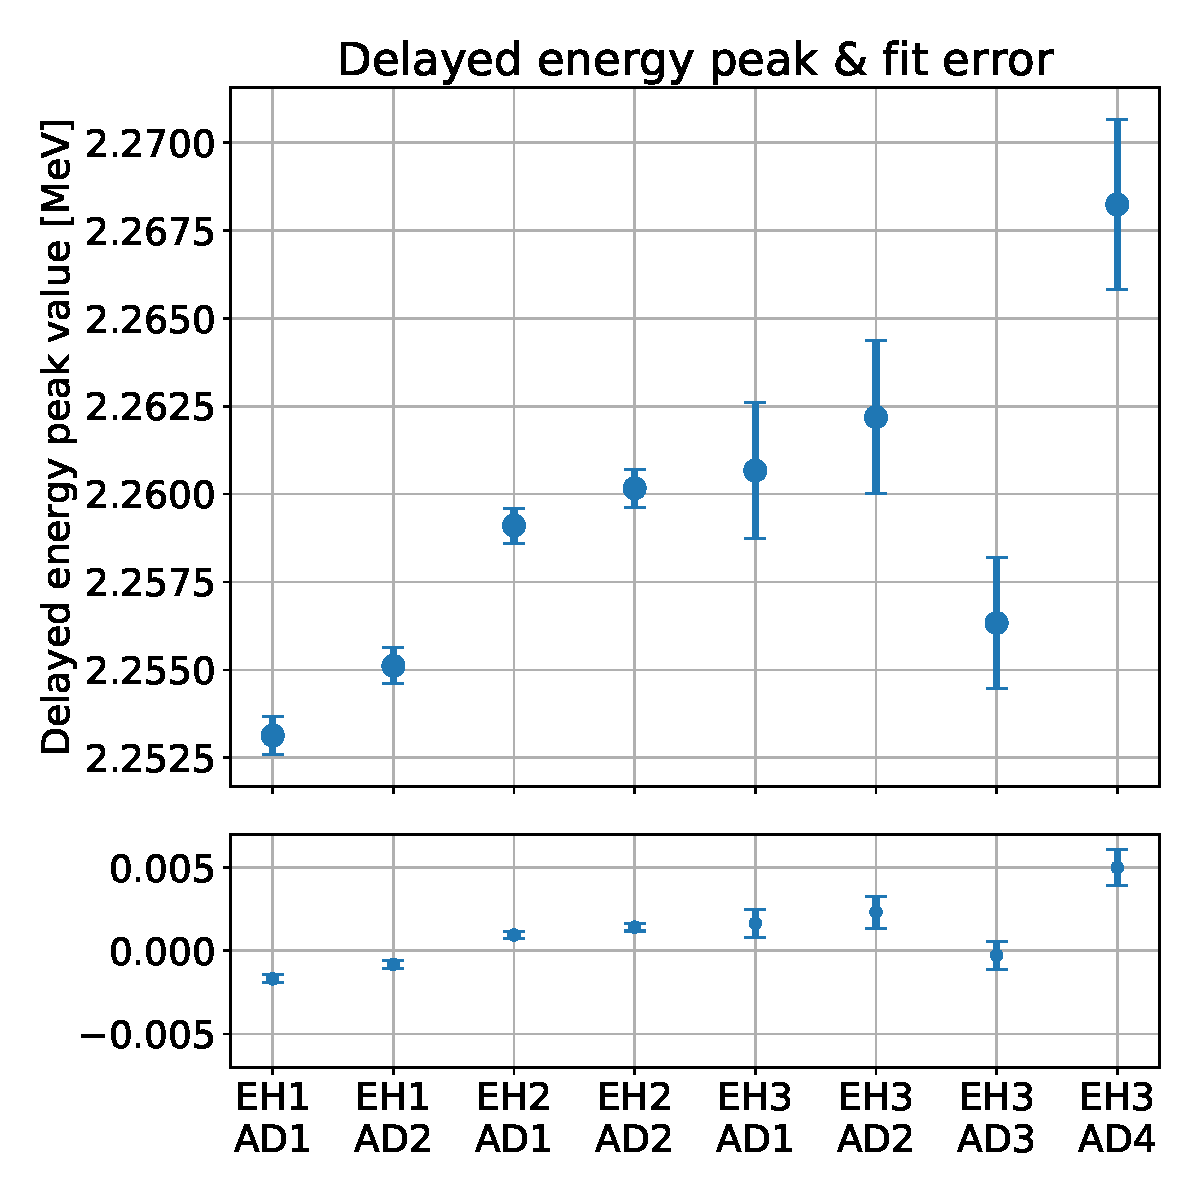
\includegraphics[height=0.33\textheight]{plot_diagnostics/delayed_energy_peak.pdf}
    \vspace{0.5cm}\hspace{0.5cm}
    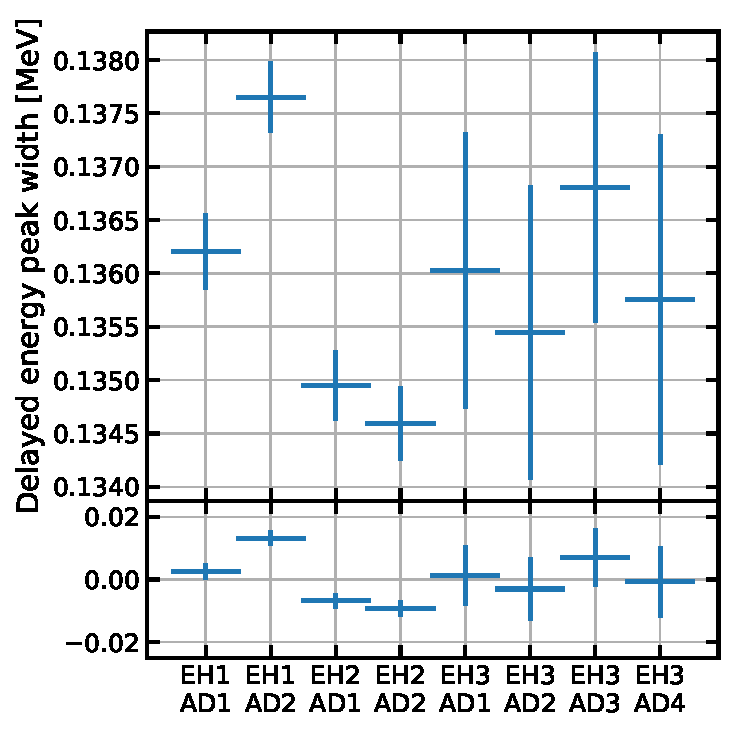
\includegraphics[height=0.33\textheight]{plot_diagnostics/delayed_energy_width.pdf}\\
    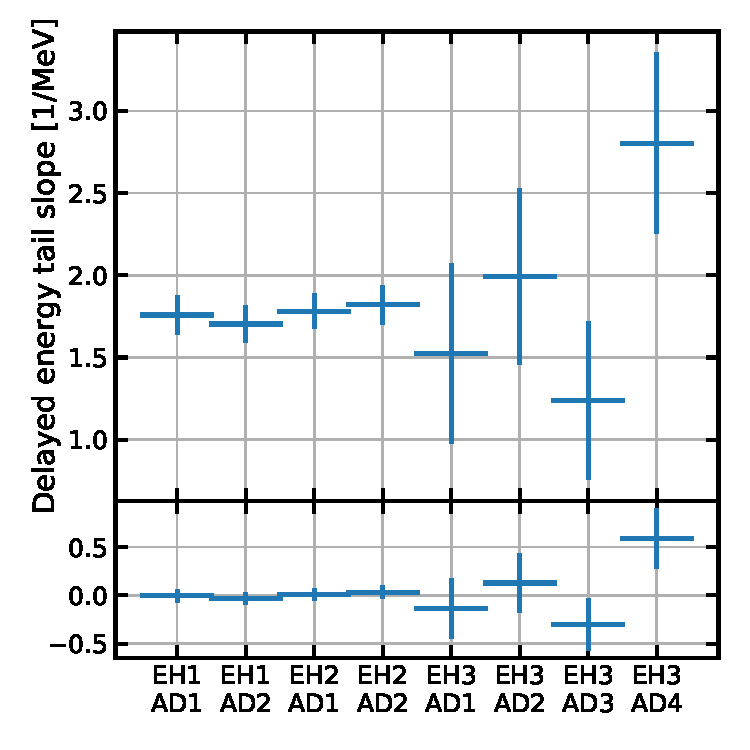
\includegraphics[height=0.33\textheight]{plot_diagnostics/delayed_energy_expo_scale.pdf}
    \hspace{0.5cm}
    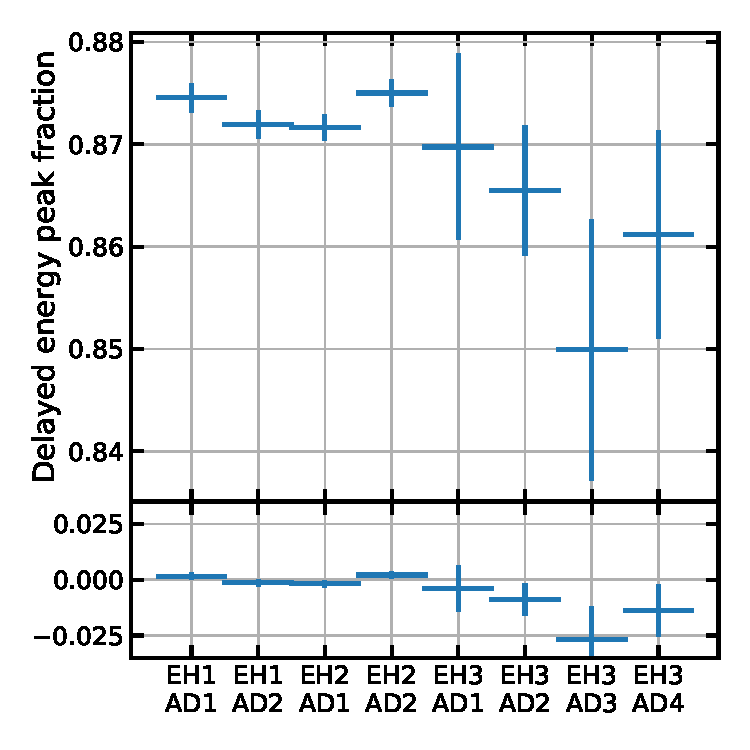
\includegraphics[height=0.33\textheight]{plot_diagnostics/delayed_energy_peak_frac.pdf}\\
    \caption{
        Fit parameters for each AD.
        Error bars represent fit errors.
        The smaller plots show the relative deviation of each AD's value
        from the average value of the 4 near-hall ADs.
    }

    \label{fig:delayed_fit_parameters}
\end{figure}

\begin{table}[ht]
    \centering
    \begin{tabular}[t]{lllll}
        \hline
        & Peak energy [\si{\mev}]
        & Width [\si{\mev}]
        & Tail slope [\si{\per\mev}]
        & Peak fraction \\
        \hline
        EH1-AD1 & \num{2.2531} & \num{0.1365} & \num{1.6893} & \num{0.8683}\\
        EH1-AD2 & \num{2.2551} & \num{0.1380} & \num{1.6247} & \num{0.8666}\\
        EH2-AD1 & \num{2.2591} & \num{0.1351} & \num{1.7212} & \num{0.8663}\\
        EH2-AD2 & \num{2.2602} & \num{0.1348} & \num{1.7319} & \num{0.8902}\\
        \hline
        EH3-AD1 & \num{2.2607} & \num{0.1360} & \num{1.5812} & \num{0.8667}\\
        EH3-AD2 & \num{2.2622} & \num{0.1349} & \num{2.1516} & \num{0.8616}\\
        EH3-AD3 & \num{2.2563} & \num{0.1366} & \num{1.3432} & \num{0.8507}\\
        EH3-AD4 & \num{2.2682} & \num{0.1362} & \num{2.5653} & \num{0.8617}\\
        \hline
    \end{tabular}
    \caption{Delayed energy fit parameters}
    \label{tab:delayed_fit_params}
\end{table}

\begin{table}[ht]
    \centering
    \begin{tabular}[t]{lll}
        \hline
        & Lower bound [\si{\mev}]
        & Upper bound [\si{\mev}] \\
        \hline
        EH1-AD1 & \num{1.8435} & \num{2.6628}\\
        EH1-AD2 & \num{1.8412} & \num{2.6690}\\
        EH2-AD1 & \num{1.8537} & \num{2.6645}\\
        EH2-AD2 & \num{1.8558} & \num{2.6646}\\
        \hline
        EH3-AD1 & \num{1.8527} & \num{2.6686}\\
        EH3-AD2 & \num{1.8575} & \num{2.6669}\\
        EH3-AD3 & \num{1.8467} & \num{2.6660}\\
        EH3-AD4 & \num{1.8597} & \num{2.6768}\\
        \hline
    \end{tabular}
    \caption{Delayed energy cut bounds derived as $\mu \pm 3\sigma$}
    \label{tab:delayed_bounds}
\end{table}

\begin{figure}
    \centering
    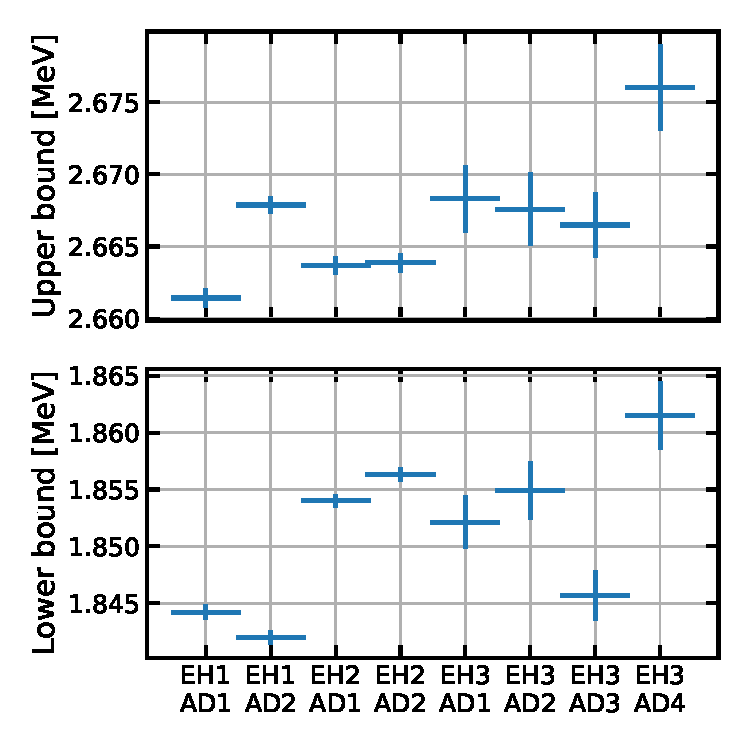
\includegraphics[height=0.40\textheight]{plot_diagnostics/delayed_energy_bounds.pdf}
    \caption{
        Delayed energy cut bounds computed as $\mu\pm 3\sigma$
        from the fitted histograms
    }
    \label{fig:delayed_bounds}
\end{figure}

The eight delayed energy spectra with their fits are shown in \cref{fig:delayed_fits}.
Comparing the fitted parameters across ADs can be used
to measure the identicalness of the ADs.
Their values and relative differences are plotted in \cref{fig:delayed_fit_parameters}
and listed in \cref{tab:delayed_fit_params}.
In particular, the top-left plot shows the relative difference
in the fitted peak $\mu$ across the ADs,
which is a measure of the energy scale variation (\cref{subsec:rel_energyscale}).
The relative variation of \SI{+-0.5}{\percent}
is used to compute the AD-uncorrelated uncertainty
on the prompt energy cut efficiency.

The bounds for the delayed energy cut are computed
based on the fitted peak value and energy resolution
from the calorimter model. The energy criterion is

\begin{equation}
    \mu - 3\sigma < E < \mu + 3\sigma.
\end{equation}
This form was decided on even though the calorimeter function
is not symmetric, and even though in reality
the detector resolution changes with energy
(and therefore is not precisely modeled in the fit).
The values used for the energy bounds are listed in \cref{tab:delayed_bounds}
and plotted in \cref{fig:delayed_bounds}.

The absolute efficiency of the delayed energy cut
is measured using Monte Carlo.
The same fitting procedure is used to establish
delayed energy cut bounds of $\mu \pm 3\sigma$ for the Monte Carlo sample.
The efficiency is then the fraction of simulated IBD events
that pass the delayed energy cut.
Note that both the numerator and denominator of the fraction includes IBD events
where the the neutron captures on other nuclei, particularly Gd.
The relative fraction of GdLS to LS therefore impacts the efficiency
because with more GdLS, fewer neutrons will capture on hydrogen.
The estimated absolute efficiency for the delayed energy cut
is \SI{\sim40}{\percent}
About half of the inefficiency is due to captures on Gd in the GdLS region,
and the other half is due to escaping $\gamma$-rays
from the LS (outer) region of the AD.
Since the absolute efficiency is not used in the \thetaot{} analysis,
a more precise value for the efficiency was not studied for this thesis.

\begin{figure}
    \centering
    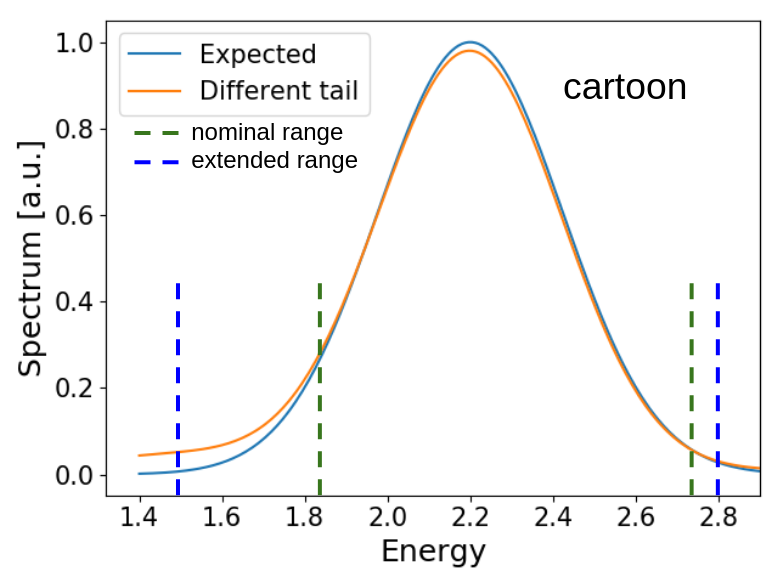
\includegraphics[height=0.4\textheight]{ch_event_selection/delayed_eff_uncertainty_cartoon}
    \caption{
        Intuition for how differences in the relative size
        of the nominal (peak) versus extended ranges
        are a proxy for differences in cut efficiency.
    }
    \label{fig:delayed_eff_unc_cartoon}
\end{figure}

The AD-uncorrelated uncertainty on the efficiency
includes variations due to all the above effects:
geometrical variations, energy scale, different material properties,
Gd fraction, etc.
The overall variation between ADs is estimated using a general method
that compares the relative size between the peak and tail regions
of the delayed energy spectrum, as defined by the delayed energy cut,
across the ADs.
Intuitively, if the same fraction of events is in the peak region in each AD,
then the cut efficiency must have a small variation.
This intuition is visualized in the cartoon in \cref{fig:delayed_eff_unc_cartoon}.
The ``expected'' curve has a high efficiency
and few events in the tail.
Since the ``different tail'' curve has more events in the tail region,
it can be concluded that this curve has a lower efficiency.

In practice, it is easier to compare the number of events in the peak
to the total number of events in an extended region that includes the tail,
rather than to just the new events in the tail.

For each AD's delayed energy spectrum, the peak region is defined as
the region passing the delayed energy cut, $\vert E-\mu \vert < 3\sigma$.
The extended region is the same for each AD:
$\SI{1.5}{\mev} < E < \SI{2.8}{\mev}$.
Using an AD-dependent definition for the peak region but
the same values for the extended creates
the desired sensitivity to variations in the energy scale.
Extending the lower bound down to \SI{1.5}{\mev} adds sensitivity to
anything that would change the shape of the tail
or the fraction of $\gamma$'s that (partially) escape from the AD.

\begin{figure}
    \centering
    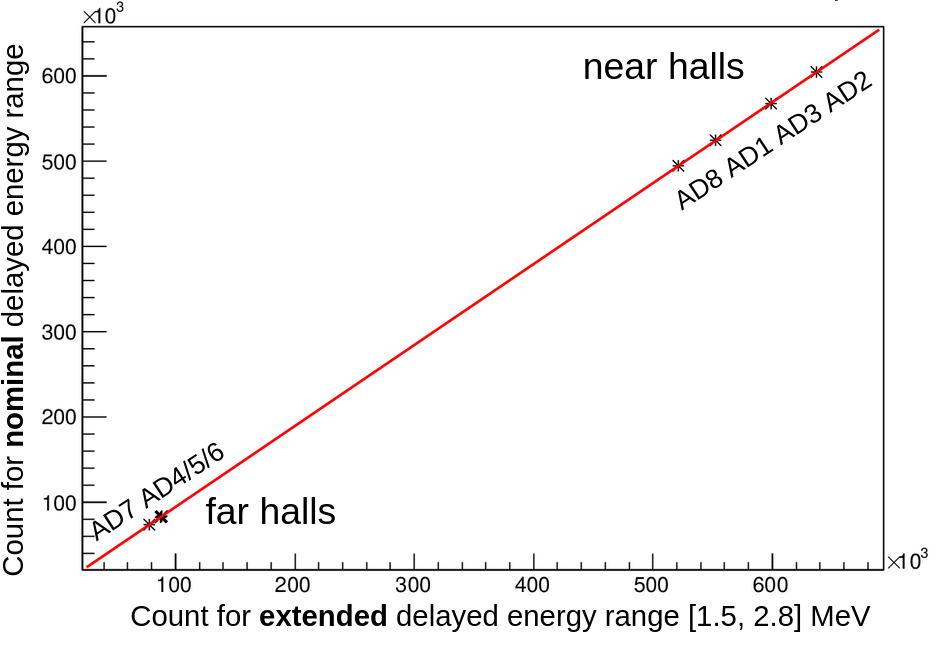
\includegraphics[height=0.4\textheight]{ch_event_selection/delayed_uncertainty_fit}\\
    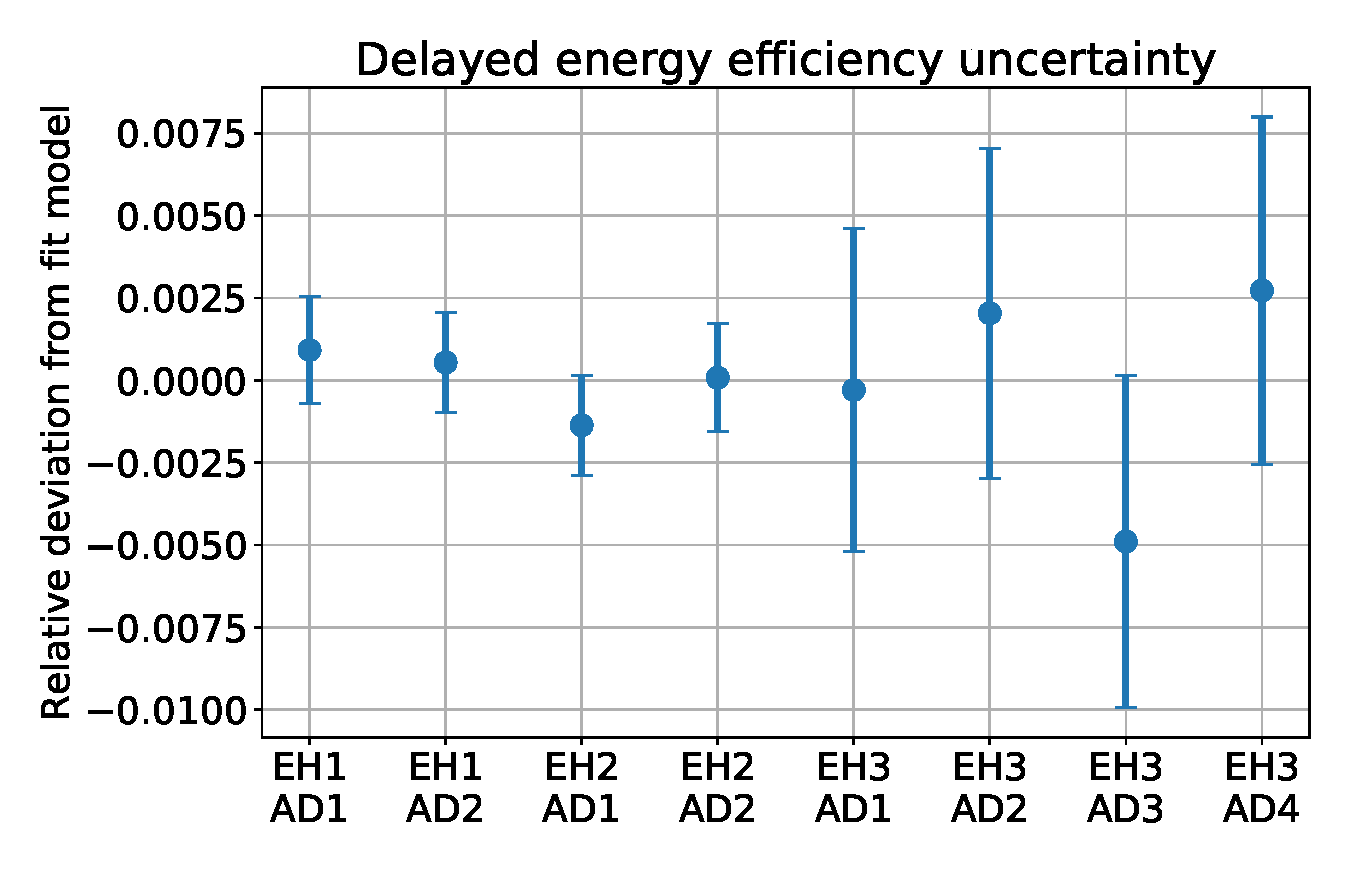
\includegraphics[height=0.4\textheight]{plot_diagnostics/delayed_energy_uncertainty_method1}
    \caption{
        (Top) Data points and (affine) linear fit
        to the number of events in the nominal (peak)
        and extended ranges of delayed energy.
        Statistical error bars are too small to be visible on this plot.
        The points are labeled using a shorthand AD indexing scheme:
        ADs 1 and 2 are EH1-AD1 and EH1-AD2. ADs 3 and 8 are EH2-AD1 and EH2-AD2.
        And ADs 4 through 7 are EH3-AD1 through EH3-AD4, respectively.\\
        (Bottom) Relative deviations from each hall to the fit model.
        The half-range of deviations for near-hall ADs
        is the delayed energy efficiency AD-uncorrelated uncertainty.
    }
    \label{fig:delayed_eff_unc_fit}
\end{figure}


If the delayed energy spectra have the same shape,
and if the calorimeter function is an appropriate fitting function
for determining the energy cut bounds,
then for some constant $b$ common to all ADs,
$N_{peak,\,i} = b N_{extended,\,i}$ for each AD $i$.
To test this model, an affine linear function is fit
to the values for each AD:

\begin{equation}
    N_{peak,\,pred,\,i} = a + b N_{extended,\,i},
\end{equation}
where $N_{peak,\,pred,\,i}$ is the fit function's prediction
of the actual event count in the peak ($N_{peak,\,i}$).
Plots of $N_{peak,\,i}$ vs. $N_{extended,\,i}$ and of the
relative deviation from the fitted line are shown in \cref{fig:delayed_eff_unc_fit}.
The fit value of $a$ should be $0$ if the simple model of
a linear scaling is correct.
Indeed, the fit value is $a = -323 \pm 387$
which is consistent with $0$.
The fit value for $b$ is $b = 0.9527 \pm 0.0015$,
which can be interpreted as a loose upper bound
on the delayed energy cut efficiency.
The final value for the AD-uncorrelated uncertainty
of the delayed energy efficiency is taken to be
the half-range of the relative deviations
of the near-hall ADs from the fitted line: \SI{0.11}{\percent}.
The far-hall ADs have much higher statistical uncertainty
(relative uncertainty $\approx\SI{0.5}{\percent}$),
and therefore larger fluctuations.
Validation that the far-hall ADs are not
substantially different from the near-hall ADs is obtained by
summing the counts for all 4 far-hall ADs to get
a combined relative deviation for the far hall of \SI{0.018}{\percent},
well within the uncertainty derived from the near halls.

This method for determining the variation in efficiency across ADs
does not account for every possible inefficiency.
For example, if the fraction of $\gamma$'s which totally or nearly totally
escape from the scintillating region is different in one AD,
but the distribution of $\gamma$'s which \textit{partially} escape is unchanged,
then this method would still suggest a high similarity between ADs.
An assumption of this analysis, therefore, is that any AD-to-AD variation
(in geometry, electronics, scintillator composition, etc.)
that affects the fraction of totally-escaping $\gamma$'s
would also change the fraction of partially-escaping $\gamma$'s.

\section{Irreducible correlated backgrounds}
\label{sec:correlated_bg}

Any event in the double coincidence dataset
that passed all multiplicity, distance, and energy cuts
and that was not caused by an IBD interaction followed by
neutron capture on hydrogen (nH)
was an irreducible background.
The accidental background analysis (\cref{sec:acc})
characterized the rate and spectrum of
the irreducible uncorrelated background,
but it was not sensitive to physical processes that produced
correlated prompt-delayed pairs.
These correlated backgrounds included muon-induced unstable isotopes (\cref{subsec:li9}),
muon-induced fast neutrons (\cref{subsec:fastn}),
and $\gamma$-rays from the \amc{} calibration source (\cref{subsec:amc}).

The muon-induced backgrounds were particularly pernicious
because the near halls had higher muon rates than the far hall,
and thus an intrinsically higher rate of these backgrounds.
If the backgrounds were not correctly characterized,
they would change the near-far ratio in a way that mimicked the effects of \thetaot.

\subsection{Muon-induced unstable isotopes}
\label{subsec:li9}

\todo[inline]{Good DocDB source for THU Li9}
Muon interactions with nuclei (primarily \isotope[12]{C}) in the AD
produced the unstable exotic isotopes \li{} and \he{}.
These isotopes $\beta$-decayed to neutron-unstable excited states
of \isotope[9]{Be} and \isotope[8]{Li}, respectively,
leading to a nonzero probability of a $\beta^{-}$-n coincidence \cite{kamland_li9}.
Unfortunately, the range of $\beta^-$ energies overlapped substantially
with the range of IBD prompt ($e^+$) energies,
and the neutron from a $\beta^-$-n decay behaved
exactly the same as a neutron from an IBD interaction.
Thus the \li{} and \he{} decays had the same signature as true IBDs.
Further, the lifetimes for \li{} and \he{} were
\SI{257.23}{\ms} and \SI{171.60}{\ms}, respectively,
meaning that the \SI{800}{\us} veto for AD muons
with energy below \SI{2.5}{\GeV} will almost always
\emph{not} veto the subsequent \li{} or \he{} decay.
The shower muon veto of \SI{1}{\s} still allowed acceptance of
$\sim e^{-4}$ of the associated \li{} and \he{} events.
In the following, unless otherwise stated,
\li{} will be used to mean both \li{} and \he{}.

The number of \li{} events contaminating the double coincidence sample
was determined by exploiting those events' time correlation
with the muon event which created the parent \li{} nucleus.
An alternate event selection with no post-muon veto
was performed to increase the contribution of \li{} events
in the resulting data sample.
Additionally, the prompt energy threshold
was raised to $E_p > \SI{3.5}{\MeV}$
to reduce the impact of accidental events.
Muon events were categorized into energy classes
of \SIrange{0.02}{1}{\GeV}, \SIrange{1}{2.5}{\GeV},
and \SI{>2.5}{\GeV}.
Additionally, any muon which was accompanied by
an AD event with energy between \SIlist{1.8;12}{\MeV}
during the interval of \SIrange{20}{200}{\us} following the muon
was ``tagged'' as a neutron-producing muon.
These neutron-tagged muons had an increased likelihood
of producing \li{}.
For each energy class of muon,
an additional subsample of neutron-tagged muons was also formed.

The double coincidence candidates which passed the alternate selection
were categorized based on the classification
of the most recent preceding AD muon,
and the time since the preceding muon
was saved in a histogram specific to the muon class.
Since the \li{} process was common to all of the ADs within a given hall,
the events from ADs in the same hall were combined
to improve the statistical uncertainty of the rate estimation.
A visualization of the alternate event selection
is shown in \cref{fig:li9_timeline}.

\begin{figure}
    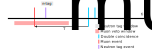
\includegraphics{ch_event_selection/timeline_li9}
    \caption{
        Event selection procedure for \li{} events.
        Neutron tags are identified within a short time window
        immediately following the muon.
        Double coincidences are only considered
        if they occur later than XYZ ms after a muon.
        The time delay between the prompt event and the muon
        is stored in a time-to-previous-muon histogram.
        \todo[inline]{Li9 timeline caption}
    }
    \label{fig:li9_timeline}
\end{figure}

The distribution of times since the preceding muon
for events correlated with muons (namely \li{})
was different from the distribution for events uncorrelated with muons
(such as IBDs or accidental backgrounds).
In particular, for muon-uncorrelated events,
the probability density for time since the preceding muon
being between $t$ and $t + dt$ was
\begin{equation}\label{eq:li9_muon_uncorr}
    p_\text{uncorr}(t) = R_\mu e^{-R_\mu t}dt,
\end{equation}
where $R_\mu$ was the rate of muon events in the particular category being examined.
Muon-correlated events had a time-since-muon distribution
which depends on both the muon rate and the decay lifetime:
\begin{equation}\label{eq:li9_muon_corr}
    p_\text{corr}(t) = \lambda_\text{iso} e^{-\lambda_\text{iso} t}dt,
\end{equation}
where $\lambda_\text{iso} = R_\mu + \nicefrac{1}{\tau_\text{iso}}$
and $\tau_\text{iso}$ is the decay time
for the muon-correlated isotope.

\begin{table}
    \centering
    \caption{Modified event selection for \li{} analysis.}
    \label{tab:li9}
    \begin{tabular}[t]{rl}
        \hline
        Post-muon veto & XYZ \si{\us} \\
        Prompt energy cut & \SI{3.5}{\MeV} \\
        Delayed energy cut & see \cref{tab:delayed_bounds} \\
        \hline
        Low-energy muon range & \SIrange{0.02}{1}{\GeV} \\
        Mid-energy muon range & \SIrange{1}{2.5}{\GeV} \\
        High-energy muon range & \SI{>2.5}{\GeV} \\
        \hline
        Neutron tag event time & \SIrange{20}{200}{\us} after muon \\
        Neutron tag event energy & \SIrange{1.8}{12}{\MeV} \\
        \hline
    \end{tabular}
\end{table}

At very short times since the preceding muon,
there was an additional muon-correlated signal
which, unlike \li{}, did decay away completely
during the nominal muon veto windows.
This signal consisted of accidental coincidences
of two \boron{} decays,
which were known to be produced in large quantities
during muon events \cite{kamland_li9}
and had a lifetime of \SI{20.2}{\ms}.
The distribution of time since the preceding muon
for \boron{}-\boron{} accidental coincidences
had the same form as \cref{eq:li9_muon_corr},
except that $\lambda_\text{B} = R_\mu + \nicefrac{2}{\tau_{B}}$
since two \boron{} decays are required.

The measured distributions of times since the preceding muon
were each fit independently with a linear combination of the above distributions:
\begin{align}\label{eq:li9_fit_fn}
    \begin{split}
        f(t) &= N_\text{bkg} (r \lambda_\text{Li} e^{-\lambda_\text{Li} t}
        + (1-r) \lambda_\text{He} e^{-\lambda_\text{He} t}) \\
             &+ N_\text{uncorr} R_\mu e^{-R_\mu t} \\
             &+ N_\text{B} \lambda_\text{B} e^{-\lambda_\text{B} t}
    \end{split}
\end{align}
In this fit, $N_\text{bkg}, N_\text{uncorr}$, and $N_\text{B}$
were free parameters representing the number of \li{} events,
number of muon-uncorrelated events (IBDs and other backgrounds),
and \boron{}-\boron{} coincidences, respectively.
The fits were not sensitive enough to extract $r$,
the fraction of the background due to \li{} rather than \he{},
so the value was fixed during the fits at \todo{Specific $r$ treatment by THU}.
A systematic uncertainty was assessed by manually varying $r$
and observing the impact on $N_\text{bkg}$.
The histograms and best-fit curves for EH1 and EH3 are shown
in \cref{fig:li9_fits}.
The histograms for EH2 are qualitatively the same as those for EH1.

\begin{figure}
    \missingfigure{\li{} fit plots}
    \caption{
        Histograms of time since the preceding muon
        at EH1 and EH3.
        The histograms for EH2 are qualitatively the same as for EH1.
    }
    \label{fig:li9_fits}
\end{figure}

For the lowest energy class (\SIrange{0.02}{1}{\GeV}),
production of \li{} was so rare that the fitter
could not effectively discriminate the \li{} events
on top of the muon-uncorrelated events (i.e. IBDs and accidentals).
Thus only the neutron-tagged sample was used to characterize this muon sample.
A systematic uncertainty was assessed on the neutron tag efficiency,
the estimated fraction of \li{} events produced by neutron-tagged muons.
The value of this efficiency was estimated by examining
the corresponding efficiency with higher-energy muons,
where it has a value of \SI{\sim60}{\percent}.
The systematic uncertainty on the neutron tag efficiency of \SI{45}{\percent}
is estimated \todo{confirm uncertainty in THU} based on the variation of the efficiency
among the higher-energy muon classes at the different experimental halls.

The extracted values for $N_\text{bkg}$ for each class of muons
were converted into the number of \li{} events
actually contaminating the neutrino candidate data sample
using the following formula:
\begin{equation}\label{eq:li9_rate_conv}
    N_\text{in data}^{\text{AD }i} =
    \frac{\varepsilon_p(\SI{1.5}{\MeV})}{\varepsilon_p(\SI{3.5}{\MeV})}
    \times
    \frac{\varepsilon_{\mu,i} T_{\text{DAQ},i}}{
        \sum_j \varepsilon_{\mu,j} T_{\text{DAQ},j}
    }
    \times
    \sum_{E\in\set{E_1,E_2,E_3}}
    \frac{N_{\text{bkg},E}}{\alpha_{ntag, E}} e^{-V_E/\tau_{\text{Li}}}
\end{equation}
The first term corrected for the different prompt energy cut
in the \li{} selection compared to the nominal IBD selection;
the efficiencies were based on the \li{} prompt spectrum computed below.
The second term divided the events for an entire hall
into portions attributed to each AD based on the nominal unvetoed livetime.
The index $j$ sums over all ADs within the same hall.
The third term is a sum of the extracted event counts
over the three muon energy classes, denoted by $E_1,E_2,E_3$.
The weighting factor $\alpha_{ntag,E}$ was equal to
the neutron tag efficiency for the low energy muon class $E_1$
where the neutron tag data sample was used to extract $N_\text{bkg}$,
and was equal to unity for the other two classes.
Lastly, the exponential term accounted for \li{} decay
over the actual muon veto windows in the nominal event selection,
which had values $V_{E1} = V_{E2} = \SI{800}{\us}$
and $V_{E3} = \SI{1}{\s}$.

The spectrum of \li{} events was computed
by comparing a \li{}-rich sample to a pure-IBD sample of events.
The \li{}-rich sample was selected as events
where the time to the preceding ``shower muon'' ($E_\mu > \SI{2.5}{\GeV}$)
was less than \SI{0.2}{\s}.
The pure-IBD sample consisted of events
where the time to the preceding muon ($E_\mu \gtrsim \SI{1.3}{\GeV}$)
was greater than \SI{1.5}{\s},
thus rejecting \SI{>99.8}{\percent} of \li{} events.
The prompt spectrum from the pure-IBD sample
was normalized to the fitted value for $N_\text{uncorr}$
and subtracted from the prompt spectrom of the \li{}-rich sample.
The resulting \li{} prompt spectrum is shown in \cref{fig:li9_spec}
and was assumed to be common among all ADs.
The prompt energy cut efficiency ratio
used to estimate the actual contamination in the neutrino candidate sample
was computed based on this spectrum.

The sources of uncertainty in the number of \li{} events
in the double coincidence data sample
can be seen in the quantities that contributed to \cref{eq:li9_rate_conv}.
The prompt energy cut efficiency ratio has an uncertainty
due to the statistical uncertainty of each bin in the extracted \li{} spectrum
(\cref{fig:li9_spec}).
No uncertainty was attributed to the livetime factor since
both the livetime and muon veto efficiency were known precisely.
The neutron tag efficiency
was the largest source of systematic uncertainty for the lowest-energy muons.
The fit result $N_\text{bkg}$ was associated with a statistical uncertainty
from the fit.

\begin{figure}
    \missingfigure{\li{} prompt spectrum}
    \caption{
        Prompt spectrum for \li{} background events.
    }
    \label{fig:li9_spec}
\end{figure}

The nH and nGd analyses used slightly different selection criteria
to measure the \li{} rate;
a detailed description of the nGd procedure can be found in \cite{chris_li9},
while the specific values used in this analysis can be found in \cite{jinjing_2020may}.


\subsection{Muon-induced fast neutrons}
\label{subsec:fastn}

Muon interactions in the rock surrounding the Daya Bay experimental halls
could produce energetic ``fast'' neutrons
which occasionally penetrated through the water pools
and into the scintillating volume in an AD.
These fast neutrons could scatter off a proton in the scintillator,
with the proton recoil causing a prompt-like scintillation signal.
When the neutron subsequently captured on a hydrogen or gadolinium nucleus,
the resulting prompt-delayed coincidence
could pass all selection criteria and contaminate the double coincidence data set.

The presence of fast neutron events in the double coincidence data set
was demonstrated by modifying the event selection
to remove the upper limit on prompt energy (nominally $E_p < \SI{12}{\MeV}$)
and examining events with prompt energy up to \SI{300}{\MeV}
(keeping all other event selection criteria intact),
as shown in [color]\todo{Update with plot} in \cref{fig:fast_neutron}.
The long tail of the spectrum was attributed to fast neutron events.
This tail provided an important constraint on the fast neutron contamination
in the nominal double coincidence data set.
The modified data set will be referred to as the
``extended double coincidence'' data set.

The number of such fast neutron events in the nominal double coincidence data set
was estimated by isolating a sample of fast neutron events
tagged by the muon system.
The resulting spectrum could be normalized based on the high-energy tail
of the modified sample's prompt energy spectrum
to provide a prediction of the rate and spectrum of fast neutron events
with lower energies.

The fast neutron events were selected by searching for
double coincidences associated with signals
in the outer water shield (OWS) of the muon system
which had no other associated muon signal
(see \cref{tab:fast_neutron}).
These events were assumed to be fast neutron events
which were caused by muons which traversed the outer water shield.
The veto for all other muons was still applied in this sample,
particularly the inner water shield (IWS) veto,
so that there was no ambiguity about whether an AD signal
was a muon or an energetic proton recoil from a fast neutron.
The OWS-tagged sample and the extended double coincidence sample for each hall
are shown in \cref{fig:fast_neutron}.
To extract the number of fast neutron events in the double coincidence sample,
the OWS-tagged sample was scaled by the normalization factor
\begin{equation}\label{eq:fast_neutron_integral}
    k_\text{fast neutron} = \frac{
        \int_{\SI{12}{\MeV}}^{\SI{300}{\MeV}} \frac{dN_{\text{extended}}}{dE} dE
    }{
        \int_{\SI{12}{\MeV}}^{\SI{300}{\MeV}} \frac{dN_{\text{OWS}}}{dE} dE
    },
\end{equation}
where the ``extended'' term refers to the histogram of prompt energies
of the extended double coincidence sample,
and the ``OWS'' term refers to the histogram for the OWS-tagged sample.
The integral notation is used for simplicity,
but in practice the bins are summed over as $\sum_i N(E_i)$.
As shown in \cref{fig:fast_neutron},
there is very good agreement in the shape of the two spectra.
The number of fast neutrons in the nominal double coincidence sample
is estimated as the number of events in the normalized OWS-tagged histogram
over the nominal prompt energy range of \SIrange{1.5}{12}{\MeV}:
\begin{equation}\label{eq:fast_neutron_count}
    N_\text{fast neutron} = k_\text{fast neutron}
    \int_{\SI{1.5}{\MeV}}^{\SI{12}{\MeV}} \frac{dN_{\text{OWS}}}{dE} dE.
\end{equation}

\begin{table}
    \centering
    \caption{
        Modified event selection criteria for the OWS-tagged
        double coincidence sample.
    }
    \label{tab:fast_neutron}
    \begin{tabular}[t]{rl}
        \hline
        Prompt energy & \SIrange{1.5}{301.5}{\MeV} \\
        Delayed energy & see \cref{tab:delayed_bounds} \\
        Time from OWS muon to prompt signal & \SI{<0.3}{\us} \\
        Time from any other muon to prompt signal & \SI{>1200}{\us} \\
        \hline
    \end{tabular}
\end{table}

\begin{figure}
    \missingfigure{Fast neutron OWS + extended plots}
    \caption{
        Prompt energy spectra for each hall
        showing the extended double coincidences
        and the OWS-tagged sample.
        The OWS-tagged sample has been normalized
        so that its integral from X to Y MeV
        matches the same integral in the extended double coincidence sample.
        \todo[inline]{Fast neutron plot caption}
    }
    \label{fig:fast_neutron}
\end{figure}

\begin{figure}
    \missingfigure{Fast neutron fit plot}
    \caption{
        Prompt energy spectra of the OWS-tagged
        and extended double coincidence samples.
        The solid curved line shows the best fit
        to the extended double coincidence sample's
        high energy range,
        extrapolated to the lower-energy (nominal) range.
    }
    \label{fig:fast_neutron_fit}
\end{figure}

The uncertainty in this estimate was computed from three sources
based on a parametri\-zation of the shape of the OWS-tagged spectrum
using a modified power law function:
\begin{equation}\label{eq:fast_neutron_powerlaw}
    \frac{dN}{dE} = N_0 \left(\frac{E}{E_0}\right)^{-a-\frac{E}{E_0}}.
\end{equation}
This function was fit to the extended double coincidence spectrum
over the energy range \SIrange{12}{300}{\MeV}
and extrapolated to the lower-energy region,
as shown in \cref{fig:fast_neutron_fit}.
The uncertainties were derived based on the fitted function's
ability to predict the value of $N_{\text{fast neutron}}$
computed in \cref{eq:fast_neutron_count}
by integrating the fitted function to obtain $N'_\text{fast neutron}$
The three sources of uncertainty were as follows:
(1) the full range of resulting $N'$ values
when fit was performed using bin widths of \SIlist{1;2;3;4}{\MeV};
(2) the maximum value of $\vert N_\text{fast neutron} - N'_\text{fast neutron}\vert$
over the different binnings;
and (3) the uncertainty in $N'_\text{fast neutron}$ due to
the propagation of the parameter errors from the fit.
For (3), the specific bin width used was arbitrarily chosen to be \SI{2}{\MeV}.
The value $N_\text{fast neutron}$ by construction did not depend
on the modified power law function in \cref{eq:fast_neutron_powerlaw}
or the binning used to perform the fit.

\subsection{\texorpdfstring{\amcbold}{Am-C} calibration source}
\label{subsec:amc}

The \amc{} calibration sources emitted neutrons at a rate of \SI{\sim0.7}{\Hz}
to allow for calibration of the ADs' response to neutron capture events
(\cref{ch:calibration}).
When not deployed during weekly calibrations, these sources
were stored within the ACUs at the top of each AD.
The sources were designed to minimize
the potential for correlated signals to reach the scintillating volume,
e.g. by attenuating the $\alpha$ energy below the $\gamma$ production
threshold for interactions with \isotope[13]{C} \cite{ngd2016}.
However, the emitted neutrons were still able to generate
correlated signals as follows.
The prompt event consisted of an emitted neutron colliding inelastically
with a nucleus (Fe, Cr, Mn or Ni) in the stainless steel surrounding the AD and ACU,
producing $\gamma$-rays which occasionally was able to penetrate
into the AD, where it interacted in the liquid scintillator.
The neutron could subsequently capture on a (different) nucleus
in the stainless steel or within the scintillating region,
in either case producing additional $\gamma$-rays
which, again, occasionally reached the scintillator and induced delayed signals.
This was the only correlated background process
which did not necessarily involve a neutron capture on H or Gd.

The rate and prompt spectrum of the \amc{} background was determined
during a special data run with an additional intense \amc{} source
deployed on the lid of EH3-AD2 for 10 days during the summer of 2012,
as shown in \cref{fig:amc_photo}.
The double coincidences observed in EH3-AD2 showed a clear asymmetry
between the upper and lower halves of the AD,
as evidenced by the distribution of reconstructed prompt positions
shown in \cref{fig:amc_position}.
An asymmetry is visible in the blue curve (EH3-AD2)
which is not present in the red curve
(EH3-AD1, which did not have an intense \amc{} source).
The additional events in the upper half of the AD
were attributed to the intense \amc{} source creating additional background.

\begin{figure}
    \centering
    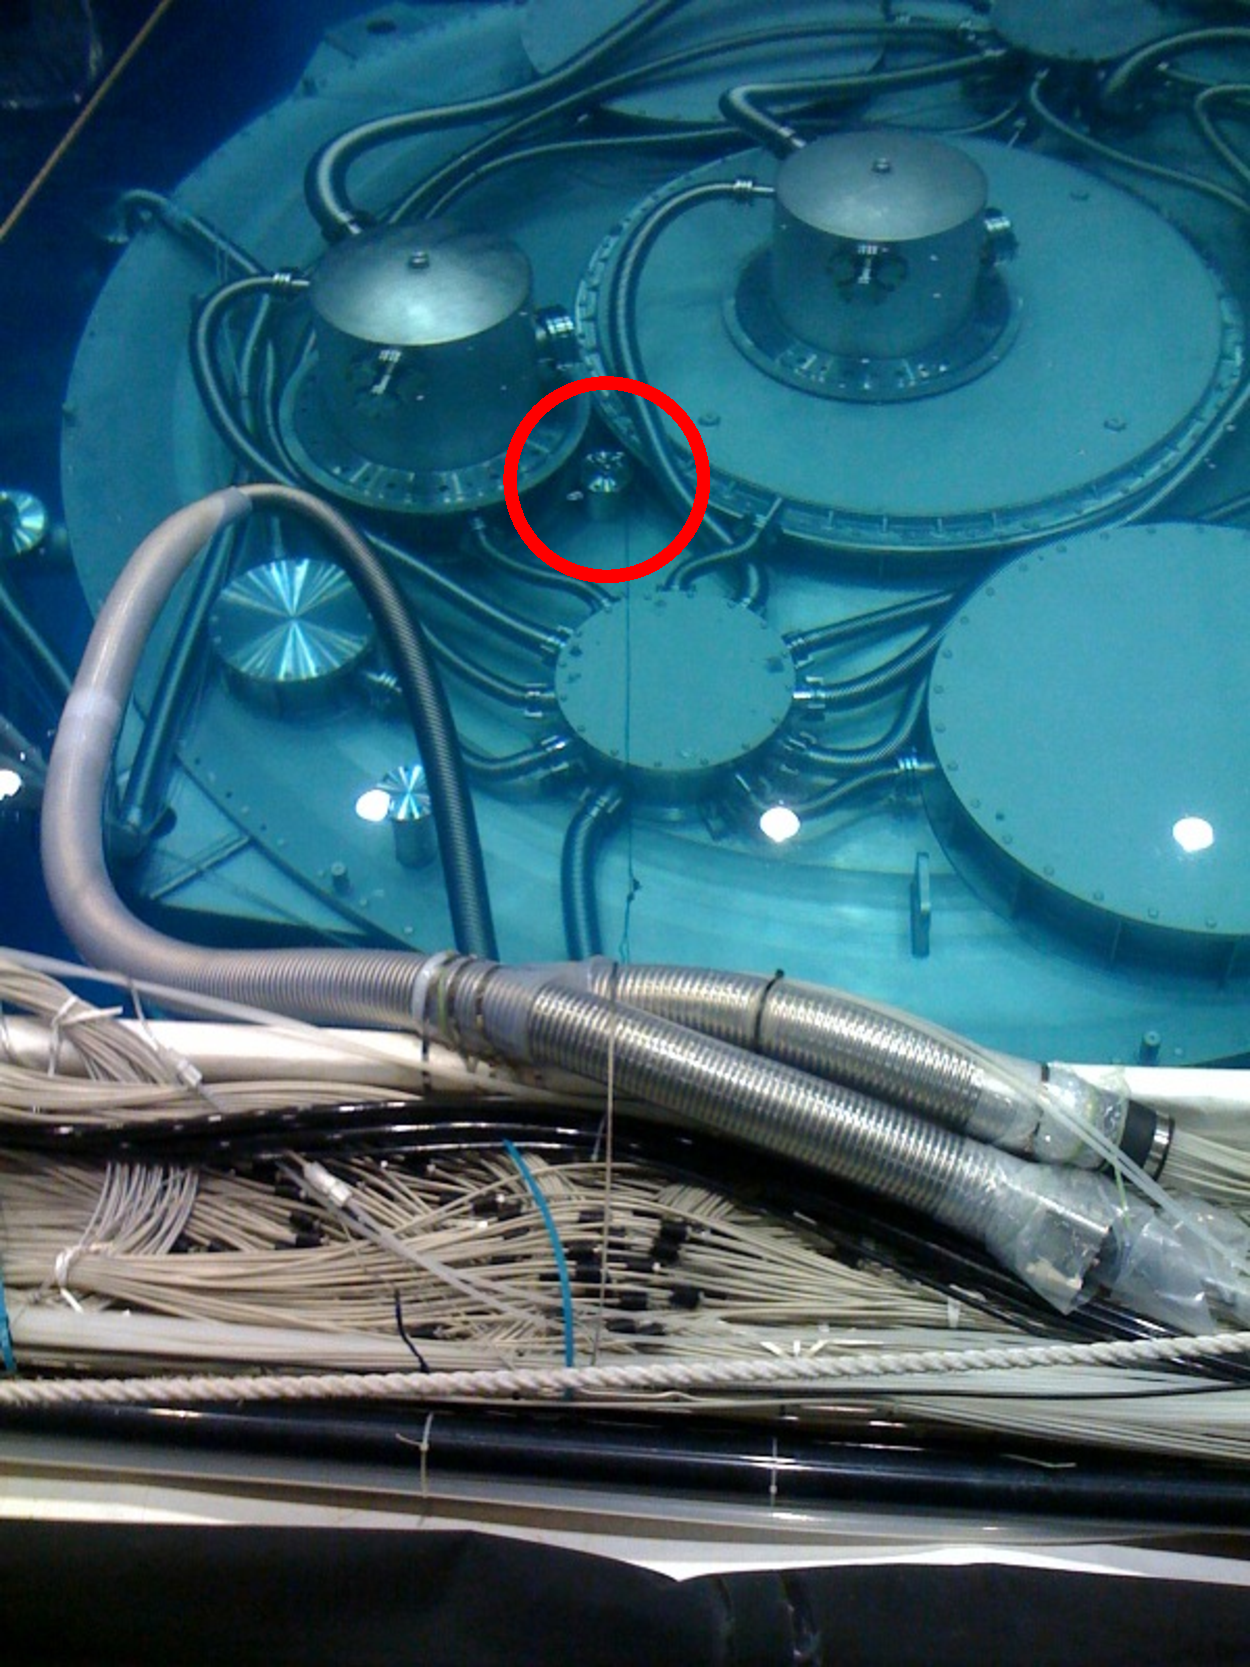
\includegraphics[width=0.5\textwidth]{ch_event_selection/amc_photo_circled}
    \caption{
        Photograph of the intense \amc{} source (circled in red)
        on the lid of EH3-AD2 between ACU-B and ACU-C \cite{amc_photo}.
    }
    \label{fig:amc_photo}
\end{figure}

A modified event selection requiring $z_\text{rec} > 0$
for both prompt and delayed events
was applied to both EH3-AD1 and EH3-AD2 data,
and the accidental background was subtracted.
(The accidental background increased in EH3-AD2 due to additional singles
from the intense \amc{} source.)
By subtracting the prompt energy distribution for EH3-AD1 from that of EH3-AD2,
the number of additional \amc{}-induced events during the intense run
was determined to be
\begin{equation}\label{eq:amc_intense}
    N_\text{int} = N_\text{EH3-AD2}(z > 0) - N_\text{EH3-AD1}(z > 0)
    = \num{121.86\pm41.89}.
\end{equation}
The prompt reconstructed energy spectrum, shown in \cref{fig:amc_spectrum},
was modeled by an exponential function,
\begin{equation}\label{eq:amc_spec_fit}
    f(E; N_0, E_0) = N_0 e^{-E/E_0}.
\end{equation}
The best-fit values were \todo{\amc{} fitted spectrum params}.

The measurement from the intense run was converted
into rates for each AD during the full data taking period
by computing a proportionality constant
relating the additional singles in the top half of an AD
(relative to the bottom half)
to the rate of \amc{} background events.
Specifically, the number of single events
with energy between \SIlist{6;12}{\MeV} was used
since the impact of the \amc{} source was larger in that range.
The proportionality constant was defined as
\begin{align}\label{eq:amc_proportion}
    \begin{split}
        \alpha_\text{AmC} &= \frac{N_\text{int}}{
            (N_\text{singles, int}(z>0) - N_\text{singles, int}(z < 0))
        }_
        {
            \SI{6}{\MeV} < E < \SI{12}{\MeV}
        } \\
        &= \frac{N_\text{int}}{N_\text{diff, int}}.
    \end{split}
\end{align}
The quantity $N_\text{diff}^{\text{AD }i}$ is defined for each AD $i$
by the same singles asymmetry measurement
given by the denominator of the first line of \cref{eq:amc_proportion}.
The estimated number of \amc{} background events
in the full nominal data sample for AD $i$ is
\begin{equation}\label{eq:amc_count}
    N_\text{AmC}^{\text{AD }i} = \alpha_\text{AmC} N_\text{diff}^{\text{AD }i}.
\end{equation}
A conservative uncertainty in the rate of \SI{50}{\percent}
was sufficient to cover the differences between the observed data
and a variety of simulations of the \amc{} background process.

\begin{figure}
    \centering
    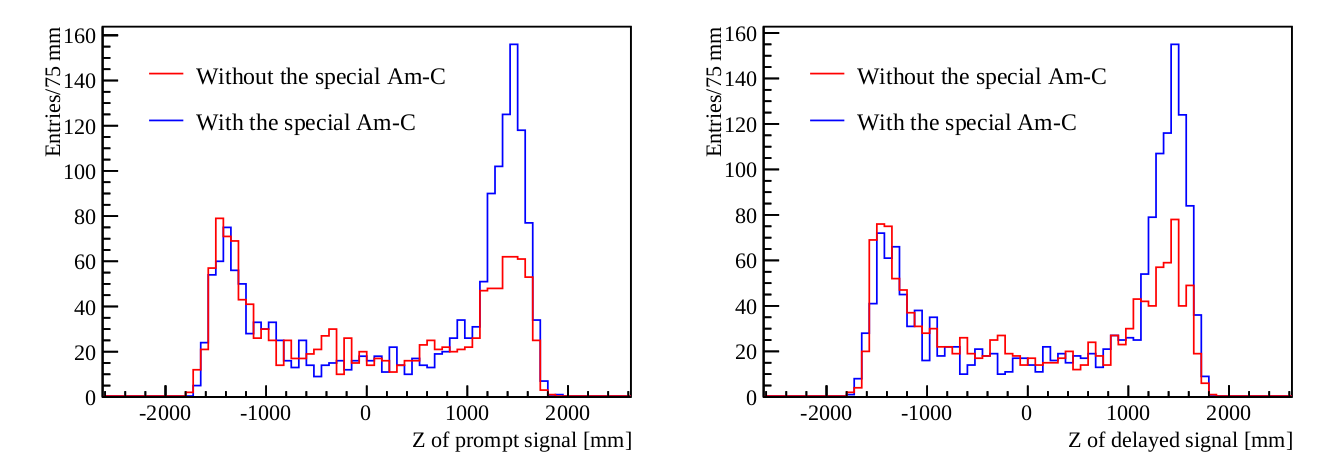
\includegraphics[width=\textwidth]{ch_event_selection/amc_position_asymmetry}
    \caption{
        Distributions of the reconstructed vertical ($z$) position
        of prompt (left) and delayed (right) signals of nH IBD candidates
        during the special \amc{} run period.
        The red line is from EH3-AD1, which did not have the special \amc{} source,
        and the blue line is from EH3-AD2, which did have the special \amc{} source.
        Figure and caption taken from \cite{nh2016technote}.
    }
    \label{fig:amc_position}
\end{figure}

\begin{figure}
    \centering
    \missingfigure{\amc{} subtracted spectrum}
    \caption{Prompt reconstructed energy spectrum.}
    \label{fig:amc_spectrum}
\end{figure}


\section{Event selection summary}
\begin{table}[ht]
    \caption{
        Event selection summary.
        The background and IBD rates are adjusted for
        $\varepsilon_\mu$ and $\varepsilon_m$.
        To convert from rates to counts, multiply by
        $T_\text{DAQ}\varepsilon_\mu\varepsilon_m$.
        The uncertainty on $N_{\text{acc}}$ and $R_{\text{acc}}$
        is only the statistical (and AD-uncorrelated) uncertainty.
        An additional \SI{0.1}{\percent} AD-correlated
        systematic uncertainty is also included in the analysis.
        The correlated background rates are taken from
        [[Jinjing's DocDB 12121 slide 30]].
        This event selection yields $\sin^22\theta_{13} = 0.06837$.
        \todo[inline]{Final event selection table \& caption}
    }
    \label{tab:summary_event_selection}
    \centering
    \tiny
    \setlength{\tabcolsep}{2.5pt}
    \sisetup{
        per-mode=reciprocal
    }
    \begin{tabular}[t]{rrrrrrrrr}  % 1 label and 8 ADs
        \hline
        & \multicolumn{2}{c}{EH1}
        & \multicolumn{2}{c}{EH2}
        & \multicolumn{4}{c}{EH3} \\
        & EH1-AD1&EH1-AD2&EH2-AD1&EH2-AD2&EH3-AD1&EH3-AD2&EH3-AD3&EH3-AD4 \\
\hline
    \end{tabular}
\end{table}
\begin{table}[ht]
    \caption{Summary of efficiency uncertainties}
    \label{tab:summary_efficiencies}
    \centering
    \begin{tabular}[t]{rr}
        \hline
        & Uncertainty (\%) \\
        \hline
    Relative energy scale uncertainty & 0.50\\
    Prompt energy cut eff. & 0.10\\
    Delayed energy cut eff. & 0.20\\
    Distance-time (DT) cut eff. & 0.50\\
\hline
    Combined cut eff. & 0.55\\
    Target proton number & 0.37\\
\hline
    Total AD-uncorrelated uncertainty & 0.66\\
    \end{tabular}
\end{table}
